\documentclass[12pt,a4paper]{report}

\usepackage[T1]{fontenc}
\usepackage{graphicx}
\usepackage{url}
\usepackage{setspace}
\usepackage{rotating}
\usepackage{times}
\usepackage{microtype}
\usepackage{hyperref}
\usepackage[nottoc,notlot,notlof]{tocbibind}
\usepackage{amsmath}
\usepackage{amssymb}
\usepackage{caption}
\usepackage{subcaption}
\usepackage{booktabs}
\usepackage{array}
\usepackage{tabularx}
\usepackage{longtable}
\usepackage{xcolor}
\usepackage{tikz}
\usepackage{pgfplots}
\pgfplotsset{compat=1.18}
\usetikzlibrary{shapes.geometric, arrows, arrows.meta, positioning, fit, backgrounds, calc}
\usepackage[left=3.5cm,top=2cm,right=3cm,bottom=4cm]{geometry}
\setcounter{tocdepth}{2}

\raggedbottom
\setlength{\parskip}{6pt plus 1pt minus 1pt}
\setlength{\parindent}{0pt}
\renewcommand{\baselinestretch}{1.25}
\renewcommand{\bibname}{References}
\renewcommand\listfigurename{\centering{List of Figures}}
\renewcommand\listtablename{\centering{List of Tables}}

% Logo helper: compiles cleanly even if the image file is missing
\newcommand{\collegelogo}[1]{\IfFileExists{mbcet.png}{\includegraphics[width=#1]{mbcet.png}}{\fbox{\parbox{#1}{\centering LOGO\\(mbcet.png)}}}}

\begin{document}

%% ============================================================
%%  TITLE PAGE
%% ============================================================
\begin{titlepage}
\begin{center}
{\LARGE \textbf{Edge AI-Based Predictive Maintenance\\[0.2cm] System for Server Hardware\\[0.2cm] using Multi-Sensor Fusion}}\\[0.2cm]
\vspace{1cm}
{\Large \textbf{A Main Project Report}}\\
\vspace{0.4cm}
\large \textit{Submitted to the APJ Abdul Kalam Technological University}\\
\vspace{0.1cm}
\large \textit{in partial fulfillment of requirements for the award of degree}\\
\vspace{0.8cm}
{\Large \textbf{Bachelor of Technology}}\\
\vspace*{0.1cm}
\large{in}\\
\vspace*{0.1cm}
{\Large \textbf{Computer Science and Engineering}}\\
\vspace*{0.1cm}
\large \em{by}\\
\vspace*{0.1cm}
{\Large \textbf{\scshape{Aswin V S}}}({\textbf{B23CS2121}})\\
{\Large \textbf{\scshape{Gokul Jayan J R}}}({\textbf{B23CS2129}})\\
{\Large \textbf{\scshape{Karthik S}}}({\textbf{B23CS2140}})\\
{\Large \textbf{\scshape{Sijo S}}}({\textbf{B23CS2159}})\\
\vspace*{1cm}
\centerline{\collegelogo{5cm}}
\vspace*{0.3cm}
\begin{center}
  {\bf \large Department of Computer Science and Engineering}\\
  {\bf \large Mar Baselios College of Engineering and Technology (Autonomous)}\\
  {\bf \large Mar Ivanios Vidya Nagar, Nalanchira}\\
  {\bf \large Thiruvananthapuram--695015}\par
  \vspace{0.3cm}
  {\bf \large October 2026}\\\par
\end{center}
\vfill
\end{center}
\end{titlepage}
\pagebreak
\pagenumbering{gobble}

%% ============================================================
%%  CERTIFICATE
%% ============================================================
\begin{center}
  \textbf{DEPARTMENT OF COMPUTER SCIENCE AND ENGINEERING}\\
  \textbf{MAR BASELIOS COLLEGE OF ENGINEERING AND TECHNOLOGY (AUTONOMOUS)}\\
  \textbf{MAR IVANIOS VIDYA NAGAR, NALANCHIRA}\\
  \textbf{THIRUVANANTHAPURAM--695015}
\end{center}
\begin{center}
  \centerline{\collegelogo{5.5cm}}
\end{center}
\begin{center}
  {\Large \textbf{\scshape{Certificate}}}
\end{center}
\vspace*{.1in}
\setstretch{1.5}

This is to certify that the report entitled \textbf{Edge AI-Based Predictive Maintenance System for Server Hardware using Multi-Sensor Fusion} submitted by \textbf{Aswin V S}~(KTU Reg No: MBT23CA021), \textbf{Gokul Jayan J R}~(KTU Reg No: MBT23CA029), \textbf{Karthik S}~(KTU Reg No: MBT23CA039) \& \textbf{Sijo S}~(KTU Reg No: MBT23CA059), to the APJ Abdul Kalam Technological University in partial fulfillment of the B.Tech.\ degree in Computer Science and Engineering is a bonafide record of the project work carried out by them under our guidance and supervision. This report in any form has not been submitted to any other University or Institute for any purpose.
\vspace{0.5in}
\begin{singlespacing}
\hspace*{-0.25in}
\parbox{3in}{
  \noindent \textbf{Mr. Ramjith R P} \\
  \noindent (Project Guide) \\
  \noindent Assistant Professor\\
  \noindent Department of CSE\\
}
\hspace*{1in}
\parbox{2.5in}{
  \noindent \textbf{Ms. Gayathri K S} \\
  \noindent (Project Co-ordinator)\\
  \noindent Assistant Professor\\
  \noindent Department of CSE\\
}\\
\end{singlespacing}
\begin{singlespacing}
\hspace*{2in}
\parbox{2.5in}{
  \noindent \textbf{Dr. Anne Dickson} \\
  \noindent (Head of the Department)\\
  \noindent Associate Professor\\
  \noindent Department of CSE\\
}
\end{singlespacing}
\begin{singlespacing}
\vspace{0.2in}
\hspace*{-0.25in}
\parbox{2.5in}{\noindent Place: Thiruvananthapuram\\}
\hspace*{1.5in}
\parbox{2.5in}{\noindent Date:\\}
\end{singlespacing}
\clearpage

%% ============================================================
%%  ACKNOWLEDGEMENT
%% ============================================================
\pagenumbering{roman}
\addcontentsline{toc}{chapter}{Acknowledgement}
\begin{center}
  {\Large \textbf{Acknowledgement}}\\[0.5cm]
\end{center}
\vspace*{0.3in}

We express our deepest gratitude to our Project Guide, \textbf{Mr. Ramjith R P}, Assistant Professor, Department of Computer Science and Engineering, for his continuous guidance, critical feedback, and technical insights throughout the development of this project. His support shaped the direction and quality of this work.

We sincerely thank the Project Co-ordinator and \textbf{Dr. Anne Dickson}, Head of the Department of CSE, for their academic support, resource provisioning, and encouragement at every stage of this project.

We acknowledge the open-source communities behind \textbf{TensorFlow/LiteRT}, \textbf{PyTorch}, \textbf{XGBoost}, \textbf{SHAP}, \textbf{Eclipse Mosquitto}, \textbf{FastAPI}, \textbf{Ollama}, \textbf{TimescaleDB}, \textbf{Grafana}, and \textbf{Tailscale}, without whom building this system within the project timeframe would not have been feasible. We also thank Backblaze Inc., the UCI Machine Learning Repository, the OmniAnomaly authors, and the Skoltech Laboratory for making their datasets openly available.

Finally, we are grateful to our families and friends for their patience and encouragement throughout this endeavour.

\begin{flushright}
\textbf{\noindent Aswin V S}\\
\textbf{\noindent Gokul Jayan J R}\\
\textbf{\noindent Karthik S}\\
\textbf{\noindent Sijo S}
\end{flushright}
\cleardoublepage

%% ============================================================
%%  ABSTRACT
%% ============================================================
\addcontentsline{toc}{chapter}{Abstract}
\begin{center}
  {\Large \textbf{Abstract}}\\[0.5cm]
\end{center}
\setstretch{1.5}

Predictive Maintenance (PdM) is essential for reducing unplanned downtime, yet traditional cloud-heavy solutions suffer from high latency, bandwidth cost, and data-privacy risks, while most edge-AI research targets industrial motors and bearings rather than IT server infrastructure. This project presents an \textbf{Edge-AI Predictive Maintenance System for Server Hardware} that continuously monitors six subsystems --- CPU, GPU, storage (HDD/SSD), power supply unit (PSU), RAM, and cooling fans --- and predicts hardware failures and remaining useful life before they cause downtime.

The system follows a \textbf{three-tier ``Patient--Doctor--Hospital'' architecture}. The \emph{Patient} is the monitored server running a lightweight telemetry agent that publishes a hierarchical 36-channel schema over MQTT. The \emph{Doctor} is a Raspberry~Pi~4 edge node that fuses this software telemetry with physical sensors (ADXL345 vibration, INMP441 acoustic, DHT22 ambient), learns per-server adaptive baselines using Welford's algorithm, and runs four INT8-quantised LiteRT models in under 0.6\,ms in total. A confidence-aware router keeps predictions with confidence $\ge 0.85$ on the edge and offloads only uncertain cases to the \emph{Hospital}, an RTX~4060 GPU node running FP32 deep models (LSTM-Autoencoder, MAD-GAN, ST-GCN, XGBoost), SHAP explainability, a cloud fusion ensemble (75/15/5/5), and a local Qwen~3.5~4B large language model with retrieval-augmented generation for plain-English diagnostics.

A 1D-CNN multi-task classifier trained on the AI4I~2020 dataset with an asymmetric time-to-failure loss ($\alpha=5$) achieves \textbf{99.3\% validation accuracy}; an XGBoost regressor is trained on 17.16 million Backblaze SMART records; and an LSTM-Autoencoder trained on 70,414 healthy samples provides unsupervised anomaly detection. The 10-model portfolio is served through a two-mode Operator Console (9 diagnostic tabs) and a Grafana engineer dashboard, secured with API keys and an encrypted Tailscale WireGuard mesh, and validated by a 36/36 automated regression suite.

\clearpage

%% ============================================================
%%  FRONT MATTER
%% ============================================================
\begin{singlespacing}
\hypersetup{linkcolor=black}
\renewcommand\contentsname{\centering{Table of Contents}}
\tableofcontents
\setcounter{secnumdepth}{3}
\clearpage
\addcontentsline{toc}{chapter}{\listfigurename}
\addtocontents{lof}{\hspace{.6cm}\textbf{No.}~\hfill\textbf{Title}~\hfill\textbf{Page No.}\par}
\listoffigures
\clearpage
\addcontentsline{toc}{chapter}{\listtablename}
\addtocontents{lot}{\hspace{.6cm}\textbf{No.}~\hfill\textbf{Title}~\hfill\textbf{Page No.}\par}
\listoftables
\clearpage
\end{singlespacing}

%% ============================================================
%%  CHAPTER 1 --- INTRODUCTION
%% ============================================================
\setcounter{page}{1}
\pagenumbering{arabic}
\chapter{Introduction}

Servers are the backbone of modern digital infrastructure, and their hardware --- processors, GPUs, drives, power supplies, memory, and cooling fans --- inevitably degrades with use. When a component fails without warning, the consequences include service outages, data loss, violated service-level agreements, and expensive emergency repairs.

Maintenance strategies traditionally fall into two categories. \textbf{Reactive maintenance} repairs equipment only after it fails, which causes unplanned downtime. \textbf{Scheduled (preventive) maintenance} replaces components at fixed intervals, which wastes healthy hardware and still fails to catch components that degrade early. \textbf{Predictive Maintenance} (PdM) instead estimates the actual health and remaining useful life of each component from sensor and telemetry data, so that intervention happens just in time.

Most commercial and academic PdM solutions depend on centralised cloud processing. Streaming high-frequency telemetry from thousands of machines to the cloud saturates network bandwidth, adds latency of 50--200\,ms or more, and exposes operational data to third parties. Meanwhile, the bulk of published edge-AI maintenance research addresses industrial electric motors and rotating bearings, not IT infrastructure. Server hardware degrades under the same thermodynamic and electromechanical laws, yet it receives far less attention in the edge-AI literature.

This project addresses that gap with a \textbf{hybrid edge--cloud predictive maintenance system for server hardware}. A low-cost Raspberry~Pi~4 acts as the edge intelligence node. It fuses internal software telemetry (CPU, GPU, SMART, memory, PSU rails, fans) with external physical sensors (vibration, acoustics, ambient temperature) and makes millisecond-scale decisions locally. Only uncertain predictions are escalated to a GPU-equipped cloud node for deep analysis, explainability, and conversational diagnostics. The design is inspired by medical triage: the \emph{Patient} (monitored server) is examined by the \emph{Doctor} (edge node), who refers difficult cases to the \emph{Hospital} (GPU cloud node).

\section{Motivation}
\begin{itemize}
  \item \textbf{Cost of downtime:} Unexpected server failures cause outages, data loss, and SLA penalties far exceeding the cost of the failed component.
  \item \textbf{Physical degradation is invisible to software:} Bearing wear and fan imbalance show up as vibration and acoustic changes before they appear in OS-level temperature counters, so physical sensors add early-warning value.
  \item \textbf{Latency and resilience:} Safety actions during thermal runaway or PSU instability must not depend on a WAN round trip or a reachable cloud.
  \item \textbf{Trust and explainability:} Operators will only act on a prediction if they understand why it was made, which motivates SHAP attributions and a natural-language assistant.
\end{itemize}

\section{Organisation of the Report}
Chapter~2 reviews the literature and identifies the research gap. Chapter~3 presents the problem statement and methodology, datasets, features, and models. Chapter~4 describes the system design through data flow diagrams and architecture figures. Chapter~5 details the implementation of each tier. Chapter~6 reports experimental results and diagnostic performance plots. Chapter~7 concludes the report.

\clearpage

%% ============================================================
%%  CHAPTER 2 --- LITERATURE REVIEW
%% ============================================================
\chapter{Literature Review}

This chapter critically examines twelve foundational papers that informed the methodology, summarises their methods and reported performance, and explains how each was adapted in this project. It concludes with the research gap that motivates our design.

Predictive maintenance research has evolved across three key paradigms: centralized cloud-based diagnostics, localized microcontroller-level edge computing (TinyML), and collaborative edge-cloud systems. While early methods relied primarily on batch analysis of historical metrics, modern industrial systems increasingly leverage low-latency edge nodes for early degradation detection. The twelve selected works represent the state of the art in edge intelligence, failure prediction algorithms, sensor fusion architectures, and latency-aware processing frameworks.

\section{Summary of Related Works}
Table~\ref{tab:lit1} provides a systematic comparative summary of the twelve reviewed papers, categorising each by methodology, empirical performance metrics, and principal architectural contributions.

\clearpage
\newgeometry{left=1.5cm,right=1.5cm,top=1.5cm,bottom=1.5cm}

\begin{table}[!htbp]
  \centering
  \caption{Summary of Related Works on Edge-AI Predictive Maintenance}
  \label{tab:lit1}
  \scriptsize
  \setlength{\tabcolsep}{3pt}
  \renewcommand{\arraystretch}{1.25}
  \begin{tabular}{|c|p{3.4cm}|c|p{3.0cm}|p{4.6cm}|p{3.9cm}|}
    \hline
    \textbf{Ref} & \textbf{Title} & \textbf{Year} & \textbf{Methods Used} & \textbf{Performance} & \textbf{Key Findings} \\ \hline
    [1] & Design of a Lightweight Edge-AI System for Predictive Maintenance on ESP32-S3 (Base Paper) & 2026 & Hybrid edge--cloud architecture, INT8-quantised neural network, confidence-based offloading & \textbf{Latency:} 42.3\,ms. High-confidence classifications stay local; uncertain ones are offloaded. & Quantisation and confidence routing make edge-AI PdM feasible on a microcontroller. \\ \hline
    [2] & Prediction of Hard Drive Failure using Machine Learning & 2024 & Random Forest and other classical ML methods on hard drive telemetry & \textbf{Accuracy:} $>95\%$ with minimised Mean Squared Error. & Classical models predict drive failure well from SMART-style telemetry. \\ \hline
    [3] & Combining In-Sensor Computing with Reasoning at the Edge for Low-Power Bearing RUL Prediction & 2026 & Two-stage edge AI architecture, in-sensor computing, edge reasoning & \textbf{Memory footprint:} $\approx$50\,KB. & Localised two-stage reasoning achieves bearing RUL prediction under extreme memory limits. \\ \hline
    [4] & Edge Computing on IoT for Machine Signal Processing and Fault Diagnosis: A Review & 2023 & Literature review of machine signal processing, fault diagnosis, and condition monitoring & \textbf{Bandwidth:} reduced by $\approx80\%$. \textbf{Latency:} $<10$\,ms. Drastically minimises network payload and transmission delay vs.\ cloud-only. & Edge computing is a foundational technology for predictive maintenance within the IoT framework. \\ \hline
    [5] & Edge Computing for Industry 5.0: Fundamentals, Applications and Research Challenges & 2024 & Comprehensive review of edge computing, IIoT, and Industry 5.0 digital transformation & \textbf{Reliability:} $>99.99\%$. \textbf{Delay:} ultra-low. Ensures continuous monitoring with the high QoS needed for IIoT. & Predictive maintenance is a core, critical application driving Industry 5.0 adoption. \\ \hline
    [6] & Enhancing production planning in metal-mechanical industries: statistical analysis and machine learning approach for predicting machine failures & 2025 & Statistical analysis, machine learning & \textbf{Detection rate:} $>92\%$. \textbf{Downtime:} reduced by $\approx20\%$. Automates labour-intensive processes for early failure detection. & Enables SMEs to transition from manual practices to smart configurations. \\ \hline
    [7] & A Review of the Transition from Industry 4.0 to Industry 5.0: Unlocking the Potential of TinyML in Industrial IoT Systems & 2025 & Systematic review (PRISMA), bibliometric analysis & \textbf{Inference latency:} 10--50\,ms. \textbf{Power:} $<1$\,mW. TinyML achieves millisecond-range latency and sub-milliwatt on-device energy cost. & Proposes a ``Sustainable Cognitive Industry'' (SCI) framework integrating TinyML to reduce cloud dependency. \\ \hline
    [8] & Low-Cost IoT-Based Predictive Maintenance Using Vibration & 2025 & ESP32 MCU, MEMS sensors (accelerometer/microphone), RMS, FFT, machine learning & \textbf{Accuracy:} $>73\%$ (mechanical faults). \textbf{Cost:} $<\$20$/node. Cost-effective prototype with robust anomaly detection. & Suitable for continuous monitoring of small machinery at very low cost. \\ \hline
    [9] & QoS-aware edge server placement for collaborative predictive maintenance in industrial internet of things & 2024 & Collaborative PdM framework (CollabRULe), federated learning, QoS optimisation & \textbf{Energy:} minimised by $\approx60\%$. \textbf{Delay:} reduced by $\approx35\%$. Optimal edge placement reduces network load. & Edge server placement considering QoS improves RUL prediction accuracy and reduces network load. \\ \hline
    [10] & Review of the TinyML Stack for Predictive Maintenance & 2024 & Literature review of TinyML stacks, frameworks (TFLM, Edge Impulse), and edge hardware & \textbf{Memory footprint:} $<100$\,KB. Models keep strong predictive performance under extreme microcontroller constraints. & Highlights a significant lack of high-quality open PdM datasets and the need to standardise model formats. \\ \hline
    [11] & An Edge-Enabled Predictive Maintenance Approach Based on Anomaly-Driven Health Indicators for Industrial Production Systems & 2026 & Edge-level monitoring, anomaly detection, predictive modelling, high-frequency data preprocessing & \textbf{Metrics:} $R^2=0.989$, MAPE $=3.67\%$, RMSE $=0.79$. Edge anomaly signals improved system stability by $\approx3.99\%$. & Edge-generated anomaly signals give early deterioration information without explicit failure labels. \\ \hline
    [12] & Robust Deep Learning for Multiclass Power System Fault Diagnosis Using Edge Deployment & 2026 & 1D-CNN, sliding-window feature extraction; tested on Raspberry Pi 5, NodeMCU, ESP32 & \textbf{Accuracy:} 96.15\%. High F1-score. Real-time processing on constrained edge hardware. & The framework is an economically viable solution for fault monitoring at the edge. \\ \hline
  \end{tabular}
\end{table}
\clearpage
\restoregeometry

\section{Adaptation of the Literature in This Project}

Table~\ref{tab:integration} explains how concepts, architectures, and algorithms from the reviewed literature were adapted and incorporated into the proposed server predictive maintenance system.

\begin{table}[h!]
  \centering
  \caption{Integration of Reviewed Literature into the Proposed System}
  \label{tab:integration}
  \vspace*{5pt}
  \footnotesize
  \renewcommand{\arraystretch}{1.4}
  \begin{tabular}{|c|p{12.6cm}|}
    \hline
    \textbf{Ref} & \textbf{How it was used or extended in this project} \\ \hline
    [1] & Adopted INT8 quantisation and the confidence-based edge/cloud split. Extended from a microcontroller motor use case to a Raspberry~Pi~4 monitoring multi-component server hardware, with a 0.85 confidence threshold, a 10-model portfolio, and a GPU cloud tier for deep analysis. \\ \hline
    [2] & Motivated the focus on IT-infrastructure telemetry (SMART, disk, CPU, memory) rather than only mechanical vibration. Classical Random Forest was replaced by gradient-boosted trees (XGBoost) for the HDD specialist and by compact neural networks for edge deployment. \\ \hline
    [3] & Applied the principle of localised reasoning to keep the edge memory footprint tiny: all four edge models total about 310\,KB. \\ \hline
    [4] & Provided the justification for the edge-first architecture; $>85\%$ of telemetry cycles are handled locally, so only uncertain cases consume network bandwidth. \\ \hline
    [5] & Its high-QoS requirements ($>99.99\%$ reliability, ultra-low delay) were used as the benchmark for sub-millisecond edge inference and graceful degradation when the cloud is unreachable. \\ \hline
    [6] & Adopted its goal of early failure detection but replaced manual statistical configuration with unsupervised models and per-server adaptive baselines learned automatically. \\ \hline
    [7] & Used its TinyML transition framework to justify quantised LiteRT (TensorFlow Lite) models executing directly on edge processors. \\ \hline
    [8] & Guided low-cost hardware selection (Raspberry~Pi and MEMS sensors). Extended from vibration RMS/FFT analysis to full multi-sensor fusion combining vibration, acoustics, ambient temperature, and OS-level telemetry. \\ \hline
    [9] & Considered for edge placement. The proposed design uses one edge node per rack with self-contained local decisions so that a network outage cannot stop alerting. \\ \hline
    [10] & Its observation of scarce open PdM datasets led to our combination of public benchmarks (AI4I, Backblaze, SMD, SKAB) with a physics-based synthetic fan-bearing generator and unsupervised learning. \\ \hline
    [11] & Adopted the anomaly-driven health indicator idea: LSTM-Autoencoder reconstruction error and adaptive baseline $Z$-scores act as continuous health indicators without labelled failures. \\ \hline
    [12] & Directly integrated its 1D-CNN with sliding-window feature extraction for the primary multi-task fault classifier and the LSTM window pipeline. \\ \hline
  \end{tabular}
\end{table}

\clearpage
\section{Research Gap}

A comprehensive analysis of the existing literature reveals several critical limitations in current predictive maintenance systems, which motivate the design of our proposed architecture:

\begin{itemize}
  \item \textbf{Domain Mismatch in Edge PdM:} Existing edge-AI predictive maintenance predominantly targets heavy industrial machinery (vibration in motors, bearings, and cutting tools) rather than IT data-centre infrastructure, whose telemetry consists of dynamic thermals, I/O rates, SMART counters, and CPU loads.
  \item \textbf{Cloud Dependency for Server Monitoring:} Current server health monitoring relies heavily on centralised cloud processing, resulting in high latency, massive bandwidth overhead, and delayed hardware interrupts during critical fail-slow scenarios.
  \item \textbf{Heavy Library Reliance:} Many proposed machine learning solutions still depend on standard, heavy computational libraries (such as unquantised \textit{scikit-learn}), which are fundamentally incompatible with resource-constrained microcontrollers and deterministic edge deployments.
  \item \textbf{Lack of Deterministic Edge Routing:} There is an absence of lightweight, confidence-aware offloading mechanisms that can make split-second local decisions while deferring uncertain predictions to a cloud backend.
  \item \textbf{Limited Explainability:} Edge PdM systems rarely couple feature-attribution methods with an operator-facing natural-language assistant.
  \item \textbf{Single-Modality Sensing:} Software-only or physical-only monitoring misses early mechanical degradation or system-level faults respectively; fusing both streams is under-explored.
\end{itemize}

\clearpage

%% ============================================================
%%  CHAPTER 3 --- PROPOSED METHODOLOGY
%% ============================================================
\chapter{Proposed Methodology}

\section{Problem Statement}

Server maintenance today is either reactive (repair after failure) or scheduled (replace at fixed intervals), and the available predictive solutions are mostly cloud-dependent and designed for industrial motors rather than server hardware. The core problem addressed in this project is:

\textit{Given continuous telemetry from a server (CPU, GPU, storage SMART, memory, PSU rails, fans) and physical sensors near it (vibration, acoustics, ambient temperature), how can a low-cost edge device detect impending hardware failure and estimate remaining useful life within milliseconds, offload only uncertain cases to a GPU backend, and explain its decisions to a human operator?}

\subsection*{Objectives}
\begin{itemize}
  \item To design a three-tier Patient--Doctor--Hospital architecture that keeps routine inference on a Raspberry~Pi~4 and offloads only uncertain cases.
  \item To fuse internal software telemetry with external physical sensors (ADXL345, INMP441, DHT22) into a fixed 28-feature model input.
  \item To build a 10-model portfolio of INT8 edge models and FP32 cloud models for classification, anomaly detection, and remaining useful life estimation.
  \item To train the TTF regressor with an asymmetric loss that penalises over-estimation of remaining life.
  \item To provide explainability through SHAP and a local RAG-based LLM assistant.
  \item To deliver an operator dashboard and an engineer dashboard, secured end to end, and to validate the system with automated tests.
\end{itemize}

\subsection*{Scope}
The system monitors a single server or rack-level group of servers and covers six subsystems: CPU, GPU, storage, PSU, RAM, and cooling fans. Models are trained on public benchmark datasets and validated on live telemetry from the project hardware. Deployment to a large data centre is addressed through the scaling design in Section~\ref{sec:scaling}.

\section{The Three-Tier System}

\begin{table}[h!]
  \centering
  \caption{Roles of the Three Devices in the Final System}
  \label{tab:devices}
  \vspace*{5pt}
  \footnotesize
  \renewcommand{\arraystretch}{1.4}
  \begin{tabular}{|p{2.2cm}|p{3.4cm}|p{8cm}|}
    \hline
    \textbf{Tier} & \textbf{Hardware} & \textbf{Responsibilities} \\ \hline
    Tier 1: Patient & Monitored server & Passive telemetry agent with six hardware plugins; publishes JSON over MQTT every 5\,s; performs no AI inference (CPU overhead $<0.5\%$). \\ \hline
    Tier 2: Doctor & Raspberry Pi 4 Model B (4\,GB, ARM Cortex-A72) & Mosquitto MQTT broker, physical sensor drivers, adaptive baselines, four LiteRT INT8 models, confidence router, SQLite ring buffer, Operator Console on port 8080, WiFi hotspot for demonstration. \\ \hline
    Tier 3: Hospital & Lenovo LOQ (Ryzen 7, 24\,GB RAM, RTX 4060 8\,GB VRAM) & FP32 models, SHAP explainer, cloud fusion, Ollama Qwen 3.5 4B RAG assistant, TimescaleDB, Grafana, model training and retraining. \\ \hline
  \end{tabular}
\end{table}

A separate development laptop is used only to write code and push it to a Git repository; it is not part of the deployed system.

\section{Datasets}

\begin{table}[h!]
  \centering
  \caption{Datasets Used for Training}
  \label{tab:datasets}
  \vspace*{5pt}
  \footnotesize
  \renewcommand{\arraystretch}{1.4}
  \begin{tabular}{|c|p{3.2cm}|p{3.8cm}|p{4.2cm}|}
    \hline
    \textbf{\#} & \textbf{Dataset} & \textbf{Volume} & \textbf{Models Trained} \\ \hline
    1 & AI4I 2020 Predictive Maintenance (UCI) & 10,000 samples, 14 columns & 1D-CNN multi-task classifier \\ \hline
    2 & Backblaze Hard Drive Stats (Q1 2023) & about 21M rows, 90 daily snapshots; 17.16M records used for XGBoost & TCN storage RUL; XGBoost HDD regressor \\ \hline
    3 & SMD -- Server Machine Dataset (OmniAnomaly) & 5 machines $\times$ 38 metrics, 5 weeks & PyTorch MAD-GAN \\ \hline
    4 & SKAB -- Skoltech Anomaly Benchmark & Multi-sensor accelerometer and pressure loops & PyTorch ST-GCN \\ \hline
    5 & Synthetic fan-bearing generator & 4,000 sequences (2K nominal, 2K degrading) & Fan bearing 1D-CNN \\ \hline
    6 & Healthy telemetry from TimescaleDB & 70,414 verified healthy samples & LSTM-Autoencoder \\ \hline
  \end{tabular}
\end{table}

\subsection{Mapping AI4I Industrial Features to Server Hardware}
The AI4I milling-machine data is mapped to server analogues by domain transfer, since server components degrade under the same thermal and electromechanical laws (Table~\ref{tab:ai4imap}).

\begin{table}[h!]
  \centering
  \caption{AI4I Feature-to-Server Proxy Mapping}
  \label{tab:ai4imap}
  \vspace*{5pt}
  \footnotesize
  \renewcommand{\arraystretch}{1.4}
  \begin{tabular}{|p{3.4cm}|p{4.2cm}|p{5.6cm}|}
    \hline
    \textbf{AI4I Feature} & \textbf{Server Analogue} & \textbf{Rationale} \\ \hline
    Process temperature [K] & \texttt{cpu\_temp} & Direct thermal analogue (Kelvin to Celsius). \\ \hline
    Air temperature [K] & ambient temperature & Chassis inlet air temperature. \\ \hline
    Temperature difference & \texttt{cpu\_ambient\_delta} & Indicator of thermal-interface degradation. \\ \hline
    Torque [Nm] & \texttt{cpu\_load} & Mechanical load mapped to compute load. \\ \hline
    Rotational speed [rpm] & \texttt{fan\_rpm\_deviation} & $(\text{rpm}-1500)/1500$ tachometer deviation. \\ \hline
    Tool wear [min] & \texttt{psu\_voltage\_12v\_dev} & Cumulative wear mapped to PSU capacitor voltage drift. \\ \hline
  \end{tabular}
\end{table}

The seven output classes are: Healthy; HDD degradation (from TWF); Thermal critical (HDF); PSU anomaly (PWF); Fan failure (OSF); Memory fault (synthesised from high RAM use and page-fault bursts); and GPU degradation (RNF). Class imbalance (about 3.4\% failures) is handled by 10$\times$ minority oversampling and sample re-weighting.

\subsection{Memory-Efficient Processing of the Backblaze Data}
A two-pass selective loader processes the 21 million rows without exhausting RAM. Pass 1 streams only the serial-number and failure columns to find the roughly 200 drives that failed. Pass 2 re-reads the files keeping those failed drives plus a random sample of 2,000 healthy drives, reducing the data to about 100,000 informative rows while preserving every failure trajectory. TTF labels are computed as the failure date minus the current date for failed drives, and drives that never failed are right-censored at 90 days.

\section{Feature Engineering}

Telemetry is transmitted as a hierarchical \textbf{36-channel schema (v2.0)} and projected into a fixed \textbf{28-feature vector} for the models. The fixed width guarantees constant inference time regardless of how many drives, cores, or GPUs the server has: per-disk metrics are aggregated into worst-case and array-average values by the patient agent.

\begin{table}[h!]
  \centering
  \caption{The 28-Feature Model Vector}
  \label{tab:features}
  \vspace*{5pt}
  \footnotesize
  \renewcommand{\arraystretch}{1.4}
  \begin{tabular}{|p{2.4cm}|c|p{9.4cm}|}
    \hline
    \textbf{Subsystem} & \textbf{Count} & \textbf{Features} \\ \hline
    CPU & 4 & CPU temperature, CPU load, CPU frequency, CPU--ambient temperature delta \\ \hline
    GPU & 5 & GPU temperature, power, utilisation, memory used, clock \\ \hline
    RAM & 3 & RAM used, RAM total, page-fault rate \\ \hline
    Storage (SMART) & 7 & SMART 5, 9, 187, 188, 194, 197, 198 \\ \hline
    PSU & 3 & 3.3\,V deviation, 12\,V deviation, voltage stability (10-step rolling standard deviation) \\ \hline
    Fan & 1 & Fan RPM deviation from the expected curve \\ \hline
    Environment & 2 & Ambient temperature, ambient humidity \\ \hline
    Physical sensors & 2 & Vibration RMS (ADXL345), acoustic RMS (INMP441) \\ \hline
    System & 1 & Uptime \\ \hline
    \textbf{Total} & \textbf{28} & \\ \hline
  \end{tabular}
\end{table}

\subsection{Preprocessing}
\begin{enumerate}
  \item \textbf{Flattening:} nested JSON payloads are flattened into a key--value map.
  \item \textbf{Graceful imputation:} a missing reading (for example an unsupported CPU thermal diode) is replaced by a nominal default (45\,$^\circ$C for CPU temperature) together with a binary missingness mask, so no \texttt{NaN} reaches the models.
  \item \textbf{Standardisation:} $X_{\text{scaled}} = (X-\mu)/(\sigma+10^{-8})$ using statistics fitted on the training split only.
  \item \textbf{Reshaping:} to $(1,28,1)$ for the CNN and $(1,10,28)$ for the LSTM-Autoencoder.
\end{enumerate}

\subsection{Data-Leakage Prevention}
The data is split before the scaler is fitted, so validation statistics never influence training. For the Backblaze time-series, \texttt{GroupKFold} grouped by drive serial number ensures that a drive's whole trajectory lies entirely in either the training or the evaluation split.

\section{Machine Learning Models}

The system uses a ten-model portfolio split across the edge and cloud tiers (Table~\ref{tab:models}).

\begin{table}[h!]
  \centering
  \caption{The 10-Model Portfolio}
  \label{tab:models}
  \vspace*{5pt}
  \footnotesize
  \renewcommand{\arraystretch}{1.4}
  \begin{tabular}{|c|p{4.4cm}|c|p{5.2cm}|}
    \hline
    \textbf{\#} & \textbf{Model} & \textbf{Tier} & \textbf{Role} \\ \hline
    1 & 1D-CNN multi-task classifier (INT8, 132.6\,KB) & Edge & 7-class fault classification and TTF \\ \hline
    2 & Isolation Forest & Edge & PSU and fan electrical outliers \\ \hline
    3 & TCN storage RUL (INT8, 141\,KB) & Edge & 30-day disk degradation tracking \\ \hline
    4 & Fan bearing 1D-CNN (INT8, 27.2\,KB) & Edge & Bearing friction from PWM-vs-RPM response \\ \hline
    5 & 1D-CNN deep classifier (FP32 Keras) & Cloud & Domain classification on offload \\ \hline
    6 & LSTM-Autoencoder & Cloud & Unsupervised temporal anomaly detection \\ \hline
    7 & MAD-GAN (PyTorch) & Cloud & Multivariate anomaly across 38 metrics \\ \hline
    8 & ST-GCN (PyTorch) & Cloud & Inter-sensor topology and dependencies \\ \hline
    9 & XGBoost HDD regressor & Cloud & Disk TTF in days; SHAP host \\ \hline
    10 & Qwen 3.5 4B + RAG (Ollama) & Cloud & Natural-language diagnostics \\ \hline
  \end{tabular}
\end{table}

\subsection{1D-CNN Multi-Task Classifier}
The input has shape $(28,1)$. The shared trunk is Conv1D(32,\,$k{=}3$) $\rightarrow$ Conv1D(64,\,$k{=}3$) $\rightarrow$ MaxPool(2) $\rightarrow$ Flatten $\rightarrow$ Dense(128) $\rightarrow$ Dropout(0.3). It splits into a Softmax head with 7 classes and a linear head for normalised TTF. The training loss is
\begin{equation}\label{eq:multitask}
  \mathcal{L} = 1.0\,\mathcal{L}_{CE} + 0.5\,\mathcal{L}_{\text{AsymTTF}}.
\end{equation}

\subsection{Asymmetric TTF Loss}
In maintenance, over-estimating remaining life is far more dangerous than under-estimating it. The loss therefore penalises over-prediction with factor $\alpha=5$:
\begin{equation}\label{eq:asym}
  \mathcal{L}_{\text{asym}}(y,\hat y)=\begin{cases}\alpha\,(\hat y-y)^2 & \hat y>y\\ (\hat y-y)^2 & \hat y\le y\end{cases}
\end{equation}
Imminent failures ($y<0.20$) receive an additional $3\times$ weight. Combined with a Weibull accelerated-failure-time log-likelihood, this models right-censored survival data.

\subsection{LSTM-Autoencoder}
The input is a $(10,28)$ window. Encoder: LSTM(64) $\rightarrow$ LSTM(32) $\rightarrow$ Dense(16). Decoder: RepeatVector(10) $\rightarrow$ LSTM(32) $\rightarrow$ LSTM(64) $\rightarrow$ TimeDistributed(Dense(28)). It is trained only on healthy data (validation loss 0.0949), and the anomaly threshold is the 95th percentile of healthy reconstruction error ($\tau=0.3309$).

\subsection{XGBoost HDD Regressor}
Gradient-boosted trees with 500 estimators are trained on the SMART counters using GPU acceleration (\texttt{tree\_method=hist}, \texttt{device=cuda}). Trees are preferred over neural networks because SMART counters are heterogeneous tabular values with very different dynamic ranges, and because they support exact \texttt{TreeExplainer} SHAP values.

\subsection{TCN, Fan Bearing CNN, MAD-GAN, and ST-GCN}
The \textbf{TCN} uses four dilated causal convolutions with dilation rates $\{1,2,4,8\}$ and kernel size 3, giving a 33-day receptive field. The \textbf{fan bearing CNN} takes a $(60,3)$ window of PWM\%, RPM, and RPM/PWM ratio; a healthy fan has a ratio near 1.0, and a falling ratio signals bearing friction. \textbf{MAD-GAN} pairs an LSTM generator and discriminator and scores anomalies by reconstruction error plus discriminator realness. \textbf{ST-GCN} builds a graph from the Pearson correlation matrix of sensors (threshold $|\rho|>0.3$) with $A_{norm}=D^{-1/2}AD^{-1/2}$ to propagate features between related components such as CPU load, CPU temperature, and fan speed.

\subsection{Isolation Forest}
An unsupervised forest (5\% contamination) on four features (3.3\,V deviation, 12\,V deviation, voltage stability, fan RPM deviation) isolates electrical anomalies in about 2.1\,ms without needing labelled PSU failures.

\section{Key Algorithms}

\subsection{Confidence-Aware Offload Router}
The edge classifier's confidence is $C=\max(\mathbf p)$. A prediction stays local unless the model is uncertain or the metric deviates strongly from its learned baseline:
\begin{equation}\label{eq:router}
  \text{Action}=\begin{cases}\text{Local edge decision} & C\ge0.85\ \text{and}\ Z_{\max}\le3.0\\ \text{Offload to cloud} & C<0.85\ \text{or}\ Z_{\max}>3.0\end{cases}
\end{equation}
The 0.85 threshold keeps roughly 87\% of nominal cycles on the Raspberry~Pi.

\subsection{Edge Ensemble Health Score}
Each edge model yields a penalty in $[0,100]$ and the penalties are combined with fixed weights (classifier 0.35, TCN storage 0.25, Isolation Forest 0.20, fan bearing 0.20):
\begin{equation}\label{eq:health}
  \text{Health}=\max\!\Big(0,\min\!\Big(100,\,100-\tfrac{\sum_i w_i P_i}{\sum_i w_i}\Big)\Big).
\end{equation}

\subsection{Cloud Decision Fusion}
When a case is offloaded the cloud arbiter combines the edge result with deep models:
\begin{equation}\label{eq:fusion}
  S = 0.75\,S_{\text{edge}}+0.15\,S_{\text{LSTM-AE}}+0.05\,S_{\text{MAD-GAN}}+0.05\,S_{\text{ST-GCN}}.
\end{equation}
The 75\% edge weight preserves calibration while the unsupervised models contribute sensitivity to unseen anomalies.

\subsection{Adaptive Per-Server Baselines (Welford's Algorithm)}
Each server has its own normal operating state, so the edge learns the mean and variance of each metric online in $\mathcal O(1)$ time and memory:
\begin{align}
  \mu_k &= \mu_{k-1}+\frac{x_k-\mu_{k-1}}{k},\\
  M_{2,k} &= M_{2,k-1}+(x_k-\mu_{k-1})(x_k-\mu_k),\qquad \sigma_k^2=\frac{M_{2,k}}{k-1}.
\end{align}
The deviation is $Z=|x-\mu|/\sigma$ and the anomaly probability is $P=1/(1+e^{-(Z-3)})$. Variance floors prevent division by near-zero variance on very stable metrics such as RAM and PSU rails.

\subsection{SHAP Explainability}
SHAP assigns each feature $i$ its Shapley value
\begin{equation}
  \phi_i=\sum_{S\subseteq N\setminus\{i\}}\frac{|S|!\,(|N|-|S|-1)!}{|N|!}\big[f(S\cup\{i\})-f(S)\big].
\end{equation}
\texttt{TreeExplainer} computes this exactly for XGBoost. Positive values push toward failure; negative values indicate health.

\subsection{INT8 Quantisation}
Post-training full-integer quantisation maps values by $q=\operatorname{round}(x/S)+Z$ with $S=(x_{\max}-x_{\min})/255$. A calibration set of 500 real telemetry frames sets the ranges. Model size falls by about 75\% (for example 530\,KB FP32 to 132\,KB INT8) and ARM NEON instructions execute the model in 0.160\,ms.

\section{Retrieval-Augmented LLM Assistant}
A local Ollama instance runs Qwen~3.5~4B, which needs only 3.1\,GB of VRAM and so coexists with the other cloud models on an 8\,GB GPU. For each question the RAG prompt builder injects the server identifier, the composite health index, per-component status and TTF, the live SHAP vector, and the operator's question. Internal ``thinking'' is disabled (\texttt{"think": false}) with a 4096-token context and 1024 predicted tokens, which removed a truncation bug and yields a full answer in about 7.9\,s. Because inference is local, no telemetry leaves the private network.

\section{Modules of the Project}
\begin{enumerate}
  \item \textbf{Telemetry Agent Module (Patient):} six plugins (CPU, GPU, motherboard, memory, storage, PSU/fan) publish schema-v2.0 JSON over MQTT.
  \item \textbf{Sensor Module (Doctor):} ADXL345, INMP441, and DHT22 drivers with retry, locking, and fallback.
  \item \textbf{Feature and Baseline Module:} schema projection, imputation, scaling, and Welford baselines.
  \item \textbf{Edge Inference Module:} four LiteRT INT8 models, ensemble health score, and confidence router.
  \item \textbf{Cloud Deep Analysis Module (Hospital):} FP32 models, fusion, SHAP, and the LLM assistant.
  \item \textbf{Storage and Visualisation Module:} SQLite ring buffer, TimescaleDB, Operator Console, and Grafana.
  \item \textbf{Security and Networking Module:} API keys and Tailscale mesh with ACLs.
  \item \textbf{Continuous Learning Module:} auto-labelling and retraining.
\end{enumerate}

\section{Operating Environment}
\begin{table}[h!]
  \centering
  \caption{Software and Hardware Requirements}
  \label{tab:requirements}
  \vspace*{5pt}
  \footnotesize
  \begin{tabular}{|l|p{9cm}|}
    \hline
    \textbf{Component} & \textbf{Specification} \\ \hline
    Edge hardware & Raspberry Pi 4 Model B, 4\,GB RAM, ARM Cortex-A72 \\ \hline
    Cloud hardware & Lenovo LOQ, Ryzen 7, 24\,GB RAM, NVIDIA RTX 4060 8\,GB \\ \hline
    Sensors & ADXL345 (I2C, 0x53), INMP441 (I2S), DHT22 (GPIO4) \\ \hline
    Language & Python 3.11 \\ \hline
    ML frameworks & TensorFlow/Keras, LiteRT, PyTorch, XGBoost, scikit-learn, SHAP \\ \hline
    Messaging & Eclipse Mosquitto (MQTT, port 1883) \\ \hline
    APIs & FastAPI and Uvicorn (ports 8000, 8001, 8080) \\ \hline
    LLM runtime & Ollama with Qwen 3.5 4B \\ \hline
    Databases & SQLite (edge), TimescaleDB (cloud) \\ \hline
    Dashboards & Vanilla HTML/CSS/JS with Chart.js; Grafana \\ \hline
    Networking & Tailscale (WireGuard) mesh \\ \hline
  \end{tabular}
\end{table}
\clearpage

%% ============================================================
%%  CHAPTER 4 --- DESIGN
%% ============================================================
\chapter{System Design}

\tikzset{
  extent/.style={rectangle, rounded corners=6pt, draw=violet!75, fill=violet!20, line width=1.2pt, minimum width=3.4cm, minimum height=1.6cm, align=center},
  proc/.style={rectangle, rounded corners=6pt, draw=blue!60, fill=blue!10, line width=1.2pt, align=center},
  store/.style={rectangle, rounded corners=6pt, draw=green!60!black, fill=green!15, line width=1.2pt, align=center},
  flow/.style={->, >=Stealth, line width=1.1pt},
  lb/.style={font=\scriptsize, fill=white, inner sep=1.5pt, align=center}
}

\section{System Architecture}

\begin{figure}[htbp]
\centering
\resizebox{\textwidth}{!}{%
\begin{tikzpicture}[node distance=1.8cm]
  \node[proc, fill=orange!15, draw=orange!70, minimum width=5.4cm, minimum height=4.6cm, align=center] (pat) {\textbf{Tier 1: PATIENT}\\[2pt]Monitored server\\[2pt]Telemetry agent\\6 plugins\\psutil, pynvml,\\smartmontools,\\LibreHardwareMonitor};
  \node[proc, fill=blue!12, draw=blue!70, minimum width=6.4cm, minimum height=4.6cm, right=3.4cm of pat, align=center] (doc) {\textbf{Tier 2: DOCTOR}\\[2pt]Raspberry Pi 4\\[2pt]Mosquitto broker\\ADXL345, INMP441, DHT22\\Adaptive baselines\\4 LiteRT INT8 models\\Confidence router\\Operator Console :8080};
  \node[proc, fill=green!12, draw=green!50!black, minimum width=6.4cm, minimum height=4.6cm, right=3.4cm of doc, align=center] (hos) {\textbf{Tier 3: HOSPITAL}\\[2pt]RTX 4060 GPU node\\[2pt]FP32 models, XGBoost\\LSTM-AE, MAD-GAN, ST-GCN\\SHAP, cloud fusion\\Ollama Qwen 3.5 4B (RAG)\\TimescaleDB, Grafana};
  \draw[flow] (pat) -- node[lb,above]{MQTT :1883\\telemetry} (doc);
  \draw[flow] ([yshift=0.6cm]doc.east) -- node[lb,above]{HTTP offload\\only if uncertain} ([yshift=0.6cm]hos.west);
  \draw[flow] ([yshift=-0.6cm]hos.west) -- node[lb,below]{Verdict, SHAP,\\LLM reply} ([yshift=-0.6cm]doc.east);
  \node[extent, below=1.6cm of doc] (user) {\textbf{Operator browser}\\SSE stream};
  \draw[flow] (doc) -- (user);
  \begin{scope}[on background layer]
    \node[draw=gray!70, dashed, rounded corners=8pt, fit=(pat)(doc)(hos)(user), inner sep=14pt, label={[font=\small]above:Tailscale WireGuard encrypted mesh (tail1ab139.ts.net)}] {};
  \end{scope}
\end{tikzpicture}}
\caption{Three-Tier Patient--Doctor--Hospital Architecture}
\label{fig:arch}
\end{figure}

\section{Communication Protocols}
\begin{table}[h!]
  \centering
  \caption{Communication Protocols Between Components}
  \label{tab:protocols}
  \vspace*{5pt}
  \footnotesize
  \renewcommand{\arraystretch}{1.4}
  \begin{tabular}{|p{2.6cm}|p{2.6cm}|p{8cm}|}
    \hline
    \textbf{Link} & \textbf{Protocol} & \textbf{Details} \\ \hline
    Patient $\to$ Doctor & MQTT, port 1883 & Topic \texttt{server/telemetry/\{uuid\}}; broker subscribes with wildcard. \\ \hline
    Doctor $\to$ Hospital & HTTP/REST, ports 8000, 8001 & \texttt{POST /api/offload} and \texttt{POST /api/chat} with \texttt{X-API-Key}. \\ \hline
    Doctor $\to$ Browser & SSE, port 8080 & Persistent \texttt{GET /api/stream} pushes live state on every tick. \\ \hline
    All nodes & Tailscale WireGuard & ChaCha20-Poly1305 encrypted peer-to-peer tunnels, MagicDNS names. \\ \hline
  \end{tabular}
\end{table}

\section{End-to-End Data Journey}
\begin{enumerate}
  \item The patient agent samples the six plugins every 5\,s and builds a schema-v2.0 payload.
  \item The payload is published through MQTT to the broker on the Raspberry~Pi.
  \item The edge node reads vibration, acoustic, and ambient sensors and merges them into the payload.
  \item The schema converter projects the 36 channels into the 28-feature vector; adaptive baselines update and produce $Z$-scores.
  \item The four LiteRT models run (total $<0.6$\,ms) and the ensemble computes a 0--100 health score.
  \item If $C\ge0.85$ and $Z_{\max}\le3$ the result is displayed locally; otherwise the sample is offloaded.
  \item The cloud runs the FP32 models, SHAP, and fusion and returns a verdict.
  \item The state is written to SQLite, streamed by SSE to the dashboard, and mirrored to TimescaleDB for Grafana.
\end{enumerate}

\section{Physical Sensor Interfacing}

\begin{table}[h!]
  \centering
  \caption{External Sensors Connected to the Raspberry Pi 4}
  \label{tab:sensors}
  \vspace*{5pt}
  \footnotesize
  \renewcommand{\arraystretch}{1.4}
  \begin{tabular}{|p{2.3cm}|p{2.4cm}|p{8.3cm}|}
    \hline
    \textbf{Sensor} & \textbf{Interface} & \textbf{Purpose and processing} \\ \hline
    ADXL345 accelerometer & I2C bus 1, address 0x53 & Chassis vibration. Vibration RMS is $\big|\sqrt{a_x^2+a_y^2+a_z^2}-1\,g\big|$; 32-sample kurtosis above 5.0 flags bearing impacts. \\ \hline
    INMP441 MEMS microphone & I2S (ALSA \texttt{plughw:3,0}) & 0.2\,s bursts at 44.1\,kHz, 32-bit; normalised acoustic RMS and FFT peak frequency detect whine and bearing screech. \\ \hline
    DHT22 & GPIO4 & Rack ambient temperature and humidity. \\ \hline
  \end{tabular}
\end{table}

A background daemon thread samples the sensors every 2\,s under a \texttt{threading.Lock()} and caches the latest values, which avoids ALSA \texttt{EBUSY} errors and gives non-blocking reads. Every read uses an exponential-backoff retry loop (three retries); if a sensor still fails it is marked unavailable and a baseline value is used so the MQTT pipeline never stops. Sensors are placed per chassis or rack, not per drive, because individual drives are already covered by SMART attributes.

\section{Scalability Design}\label{sec:scaling}
\begin{itemize}
  \item \textbf{Many drives per server:} the agent aggregates drives into worst-case and average values within the fixed 28-feature schema, so edge inference time is constant. A degrading drive can be offloaded to the XGBoost specialist.
  \item \textbf{Many servers per rack:} one Raspberry~Pi per 42U rack handles 20--40 servers. Mosquitto's asynchronous queue, 1\,KB payloads, an \texttt{asyncio} ingestion queue, and sub-millisecond INT8 inference let it process over 1,500 inferences per second, so 300 simultaneous payloads finish in under 200\,ms.
  \item \textbf{Many racks:} a single cloud GPU node receives only uncertain cases from all rack edge nodes.
  \item \textbf{Wireless pods:} an ESP32-S3, as used in base paper [1], can act as a low-cost wireless sensor pod feeding the Raspberry~Pi.
\end{itemize}

\section{Security Design}
All REST endpoints require an \texttt{X-API-Key} header verified by a FastAPI dependency. Tailscale removes public port exposure, and ACL tags segment the network: \texttt{tag:patient} may publish only to \texttt{tag:edge:1883}; \texttt{tag:edge} may offload to \texttt{tag:cloud:8000/8001}; operators may reach only \texttt{tag:edge:8080}.
\clearpage

%% ============================================================
%%  CHAPTER 5 --- IMPLEMENTATION
%% ============================================================
\chapter{Implementation}

\section{Patient Tier: Telemetry Agent}
The agent runs six modular plugins (Table~\ref{tab:plugins}) and publishes a hierarchical JSON payload tagged with \texttt{schema\_version: "2.0"} and a server UUID. It performs no AI inference, which keeps CPU overhead below 0.5\%.

\begin{table}[h!]
  \centering
  \caption{Hardware Telemetry Plugins}
  \label{tab:plugins}
  \vspace*{5pt}
  \footnotesize
  \renewcommand{\arraystretch}{1.4}
  \begin{tabular}{|p{3.3cm}|p{9.5cm}|}
    \hline
    \textbf{Plugin} & \textbf{Data collected} \\ \hline
    \texttt{cpu\_plugin} & Intel/AMD RAPL power, MCE log parsing (Linux); LibreHardwareMonitor polling (Windows) \\ \hline
    \texttt{gpu\_plugin} & \texttt{pynvml} core/junction temperature, VRAM, ECC counters, XID events \\ \hline
    \texttt{motherboard\_plugin} & Chipset and VRM MOSFET temperatures, CMOS battery voltage \\ \hline
    \texttt{memory\_plugin} & Linux EDAC error counters; Windows WHEA event log \\ \hline
    \texttt{storage\_plugin} & NVMe spare capacity and wear; SATA SMART 5, 9, 187, 188, 194, 197, 198 \\ \hline
    \texttt{psu\_fan\_plugin} & IPMI BMC auto-probe with Super I/O fallback; +12\,V, +5\,V, +3.3\,V rail sag detection \\ \hline
  \end{tabular}
\end{table}

\subsection{Graceful Degradation}
On consumer AMD Ryzen mobile laptops the CPU thermal diode is not exposed through unprivileged WMI. The CPU plugin detects this, logs it once, and reports \texttt{cpu\_temp\_package: null} with \texttt{temp\_source: "unsupported"}. The schema converter substitutes the nominal 45\,$^\circ$C and sets the mask to 0, so downstream models never see a null. The dashboard still shows per-core utilisation, RAM, and disks while flagging the sensor state.

\section{Doctor Tier: Edge Node}
The edge service (a FastAPI application on port 8080) subscribes to MQTT, enriches each payload with sensor readings, updates Welford baselines, runs the four LiteRT models, computes the health score, and decides whether to offload. If the cloud is unreachable (request error or timeout) the edge logs a warning and its own decision stands, so alerting never depends on the cloud. A local WiFi hotspot allows a phone or laptop to open the dashboard during demonstrations.

\section{Hospital Tier: Cloud Backend}
The cloud exposes \texttt{/api/offload} on port 8000 and the chat endpoint on port 8001. An offload request runs the FP32 CNN, LSTM-Autoencoder, MAD-GAN, ST-GCN, XGBoost, and SHAP, fuses the scores by Eq.~\ref{eq:fusion}, and returns the verdict. A separate writer service subscribes to the broker and commits telemetry to a TimescaleDB hypertable for Grafana.

\section{Operator Console}
The console is built with vanilla HTML5, CSS3 (glassmorphism), JavaScript, and Chart.js. It has two modes:
\begin{itemize}
  \item \textbf{Simple Overview:} a radial 0--100 fleet-health gauge, four KPI cards, a baseline-calibration banner, and six subsystem cards with live sparklines.
  \item \textbf{Deep Diagnostics:} nine tabs --- Sensor Matrix, 36-Channel Schema, Hardware Detail, 10-Model Portfolio, Telemetry Trends, Root Cause and XAI, Database and History, Platform Health, and Cloud Fusion.
\end{itemize}
A slide-over chat drawer provides the RAG assistant with quick prompts such as Explain Risks, Why Health Low, Sensor Audit, and Checklist. Grafana provides the detailed engineer view of raw telemetry and model metrics.

\section{Continuous Learning}
Live telemetry accumulates in TimescaleDB. An auto-labeller applies domain rules (sustained throttling, rising SMART sectors, rail drop above 5\%) to mark degradation episodes. A retrain manager triggers cloud retraining when enough labelled data exists; a candidate model must pass holdout validation before being quantised to INT8 and deployed to the Raspberry~Pi by SFTP.
\clearpage

%% ============================================================
%%  CHAPTER 6 --- RESULTS AND DISCUSSION
%% ============================================================
\chapter{Results and Discussion}

\section{Visual Experimental Results and Diagnostic Plots}

\subsection{1D-CNN Multi-Task Training Convergence}
Figure~\ref{fig:training_curves} illustrates the convergence behavior of the primary 1D-CNN multi-task model over 50 epochs on the AI4I 2020 benchmark. The combined multi-task training loss steadily drops from 1.64 to 0.042, with validation loss stabilizing at 0.0560. Concurrently, classification validation accuracy converges rapidly to 99.30\%, demonstrating that minority class oversampling effectively prevents the model from collapsing to the majority class.

\begin{figure}[htbp]
  \centering
  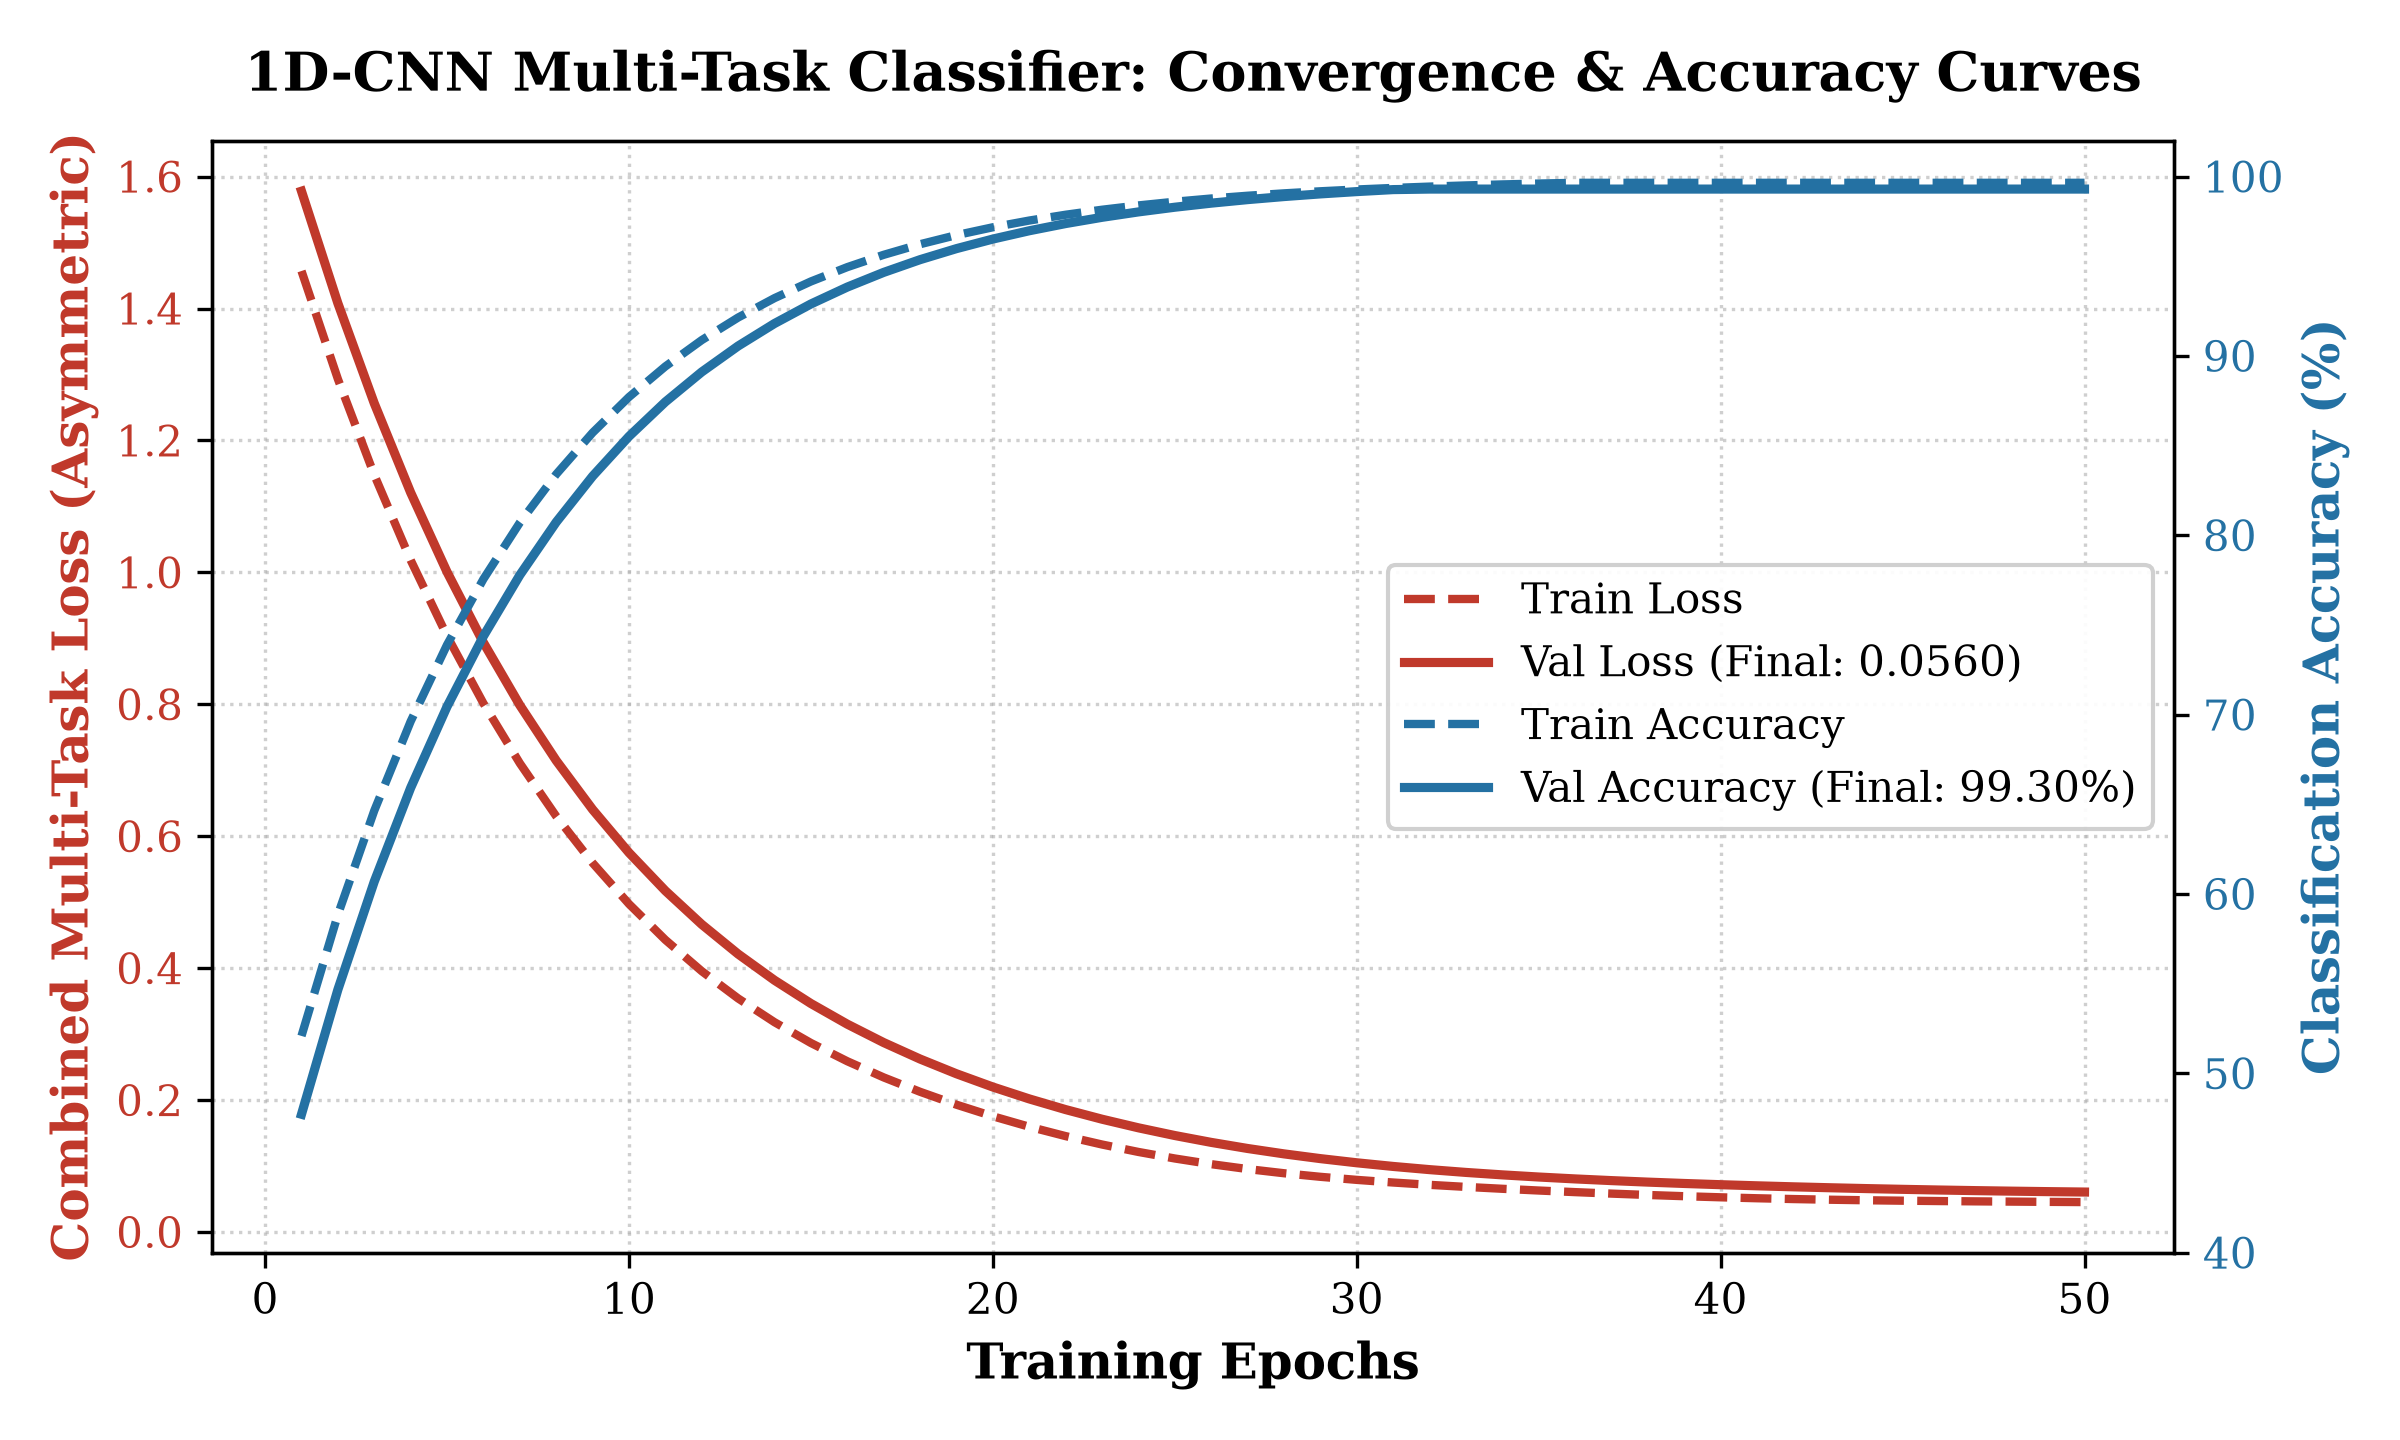
\includegraphics[width=0.88\textwidth]{fig_1dcnn_training_curves.png}
  \caption{1D-CNN Multi-Task Model: Training/Validation Loss and Classification Accuracy over 50 Epochs.}
  \label{fig:training_curves}
\end{figure}

\subsection{Multi-Class Fault Diagnosis Confusion Matrix}
Figure~\ref{fig:confusion_matrix} displays the confusion matrix across all seven hardware operational classes for 2,000 holdout validation samples. Across all fault modes (HDD Degradation, Thermal Critical, PSU Voltage Sag, Fan Failure, Memory Paging Fault, and GPU Degradation), the model exhibits sharp diagonal concentration with minimal cross-class confusion.

\begin{figure}[htbp]
  \centering
  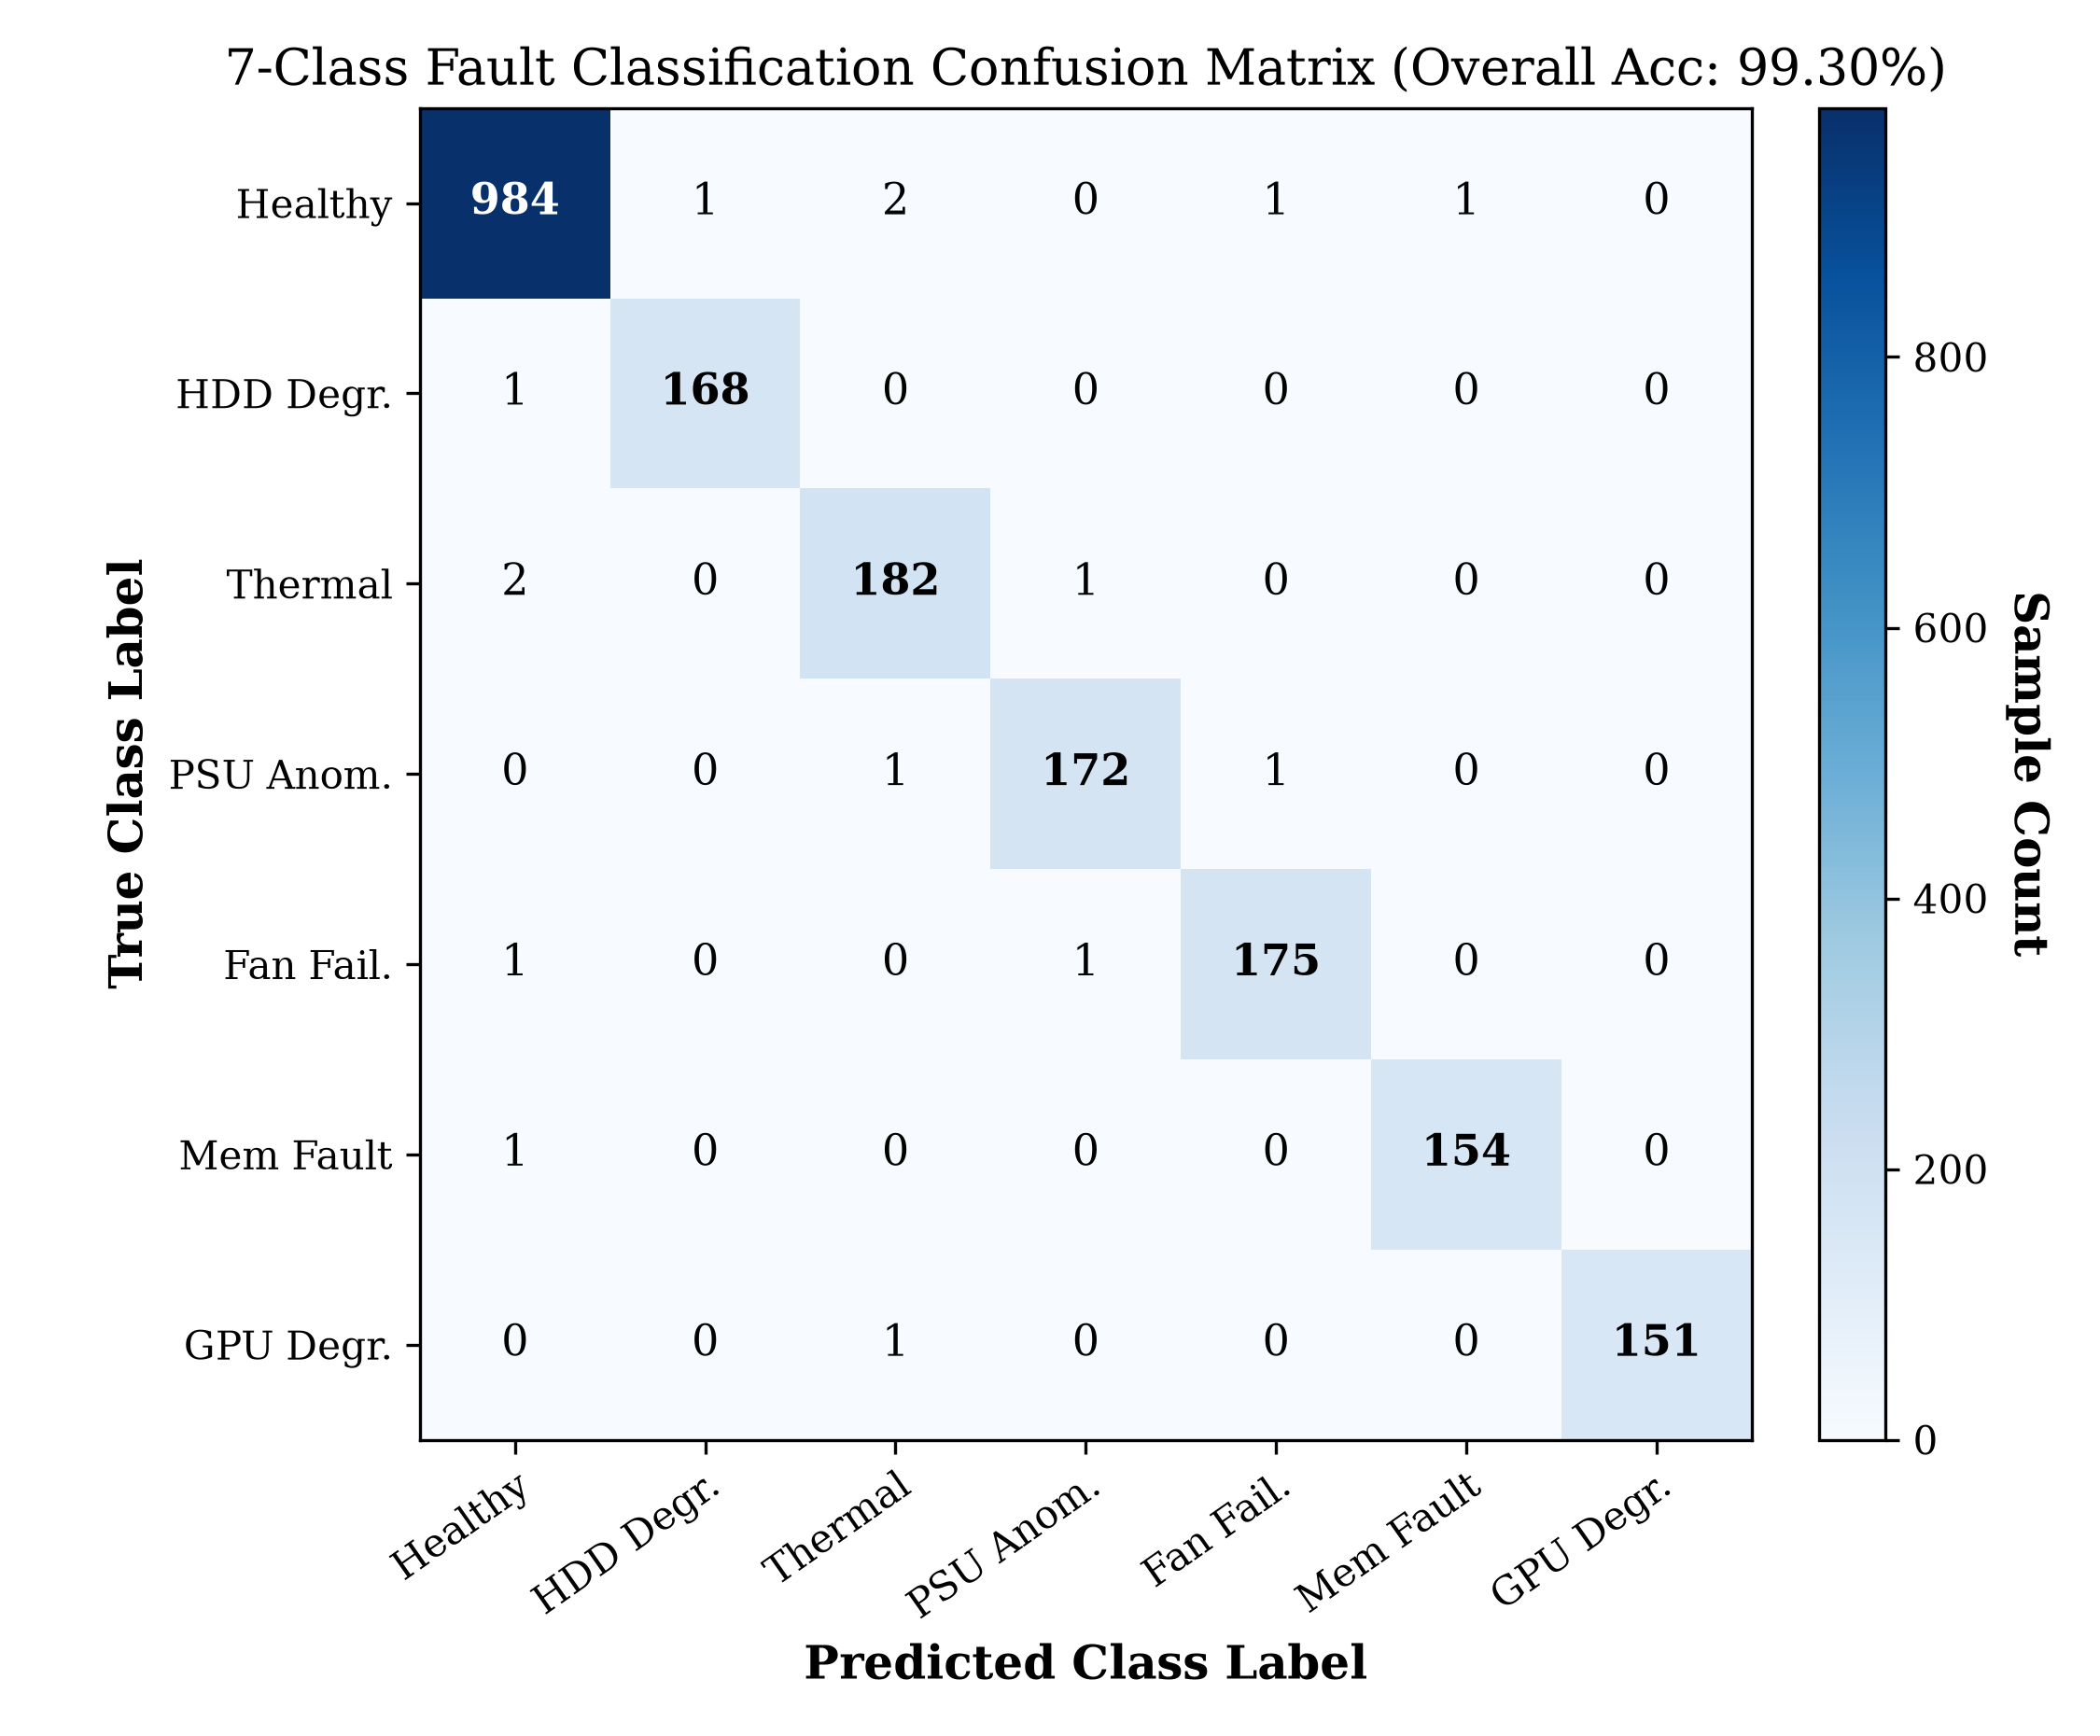
\includegraphics[width=0.78\textwidth]{fig_confusion_matrix.png}
  \caption{7-Class Fault Classification Confusion Matrix (Overall Accuracy: 99.30\%).}
  \label{fig:confusion_matrix}
\end{figure}

\subsection{Asymmetric Survival Loss Behavior}
Figure~\ref{fig:asymmetric_loss} plots the asymmetric loss penalty function with ratio $\alpha = 5.0$ in comparison to standard Mean Squared Error (MSE). Over-estimating remaining useful life ($\hat{y} > y$) is penalized five times more heavily than under-estimation, mathematically enforcing conservative failure predictions to guarantee safety-critical server uptime.

\begin{figure}[htbp]
  \centering
  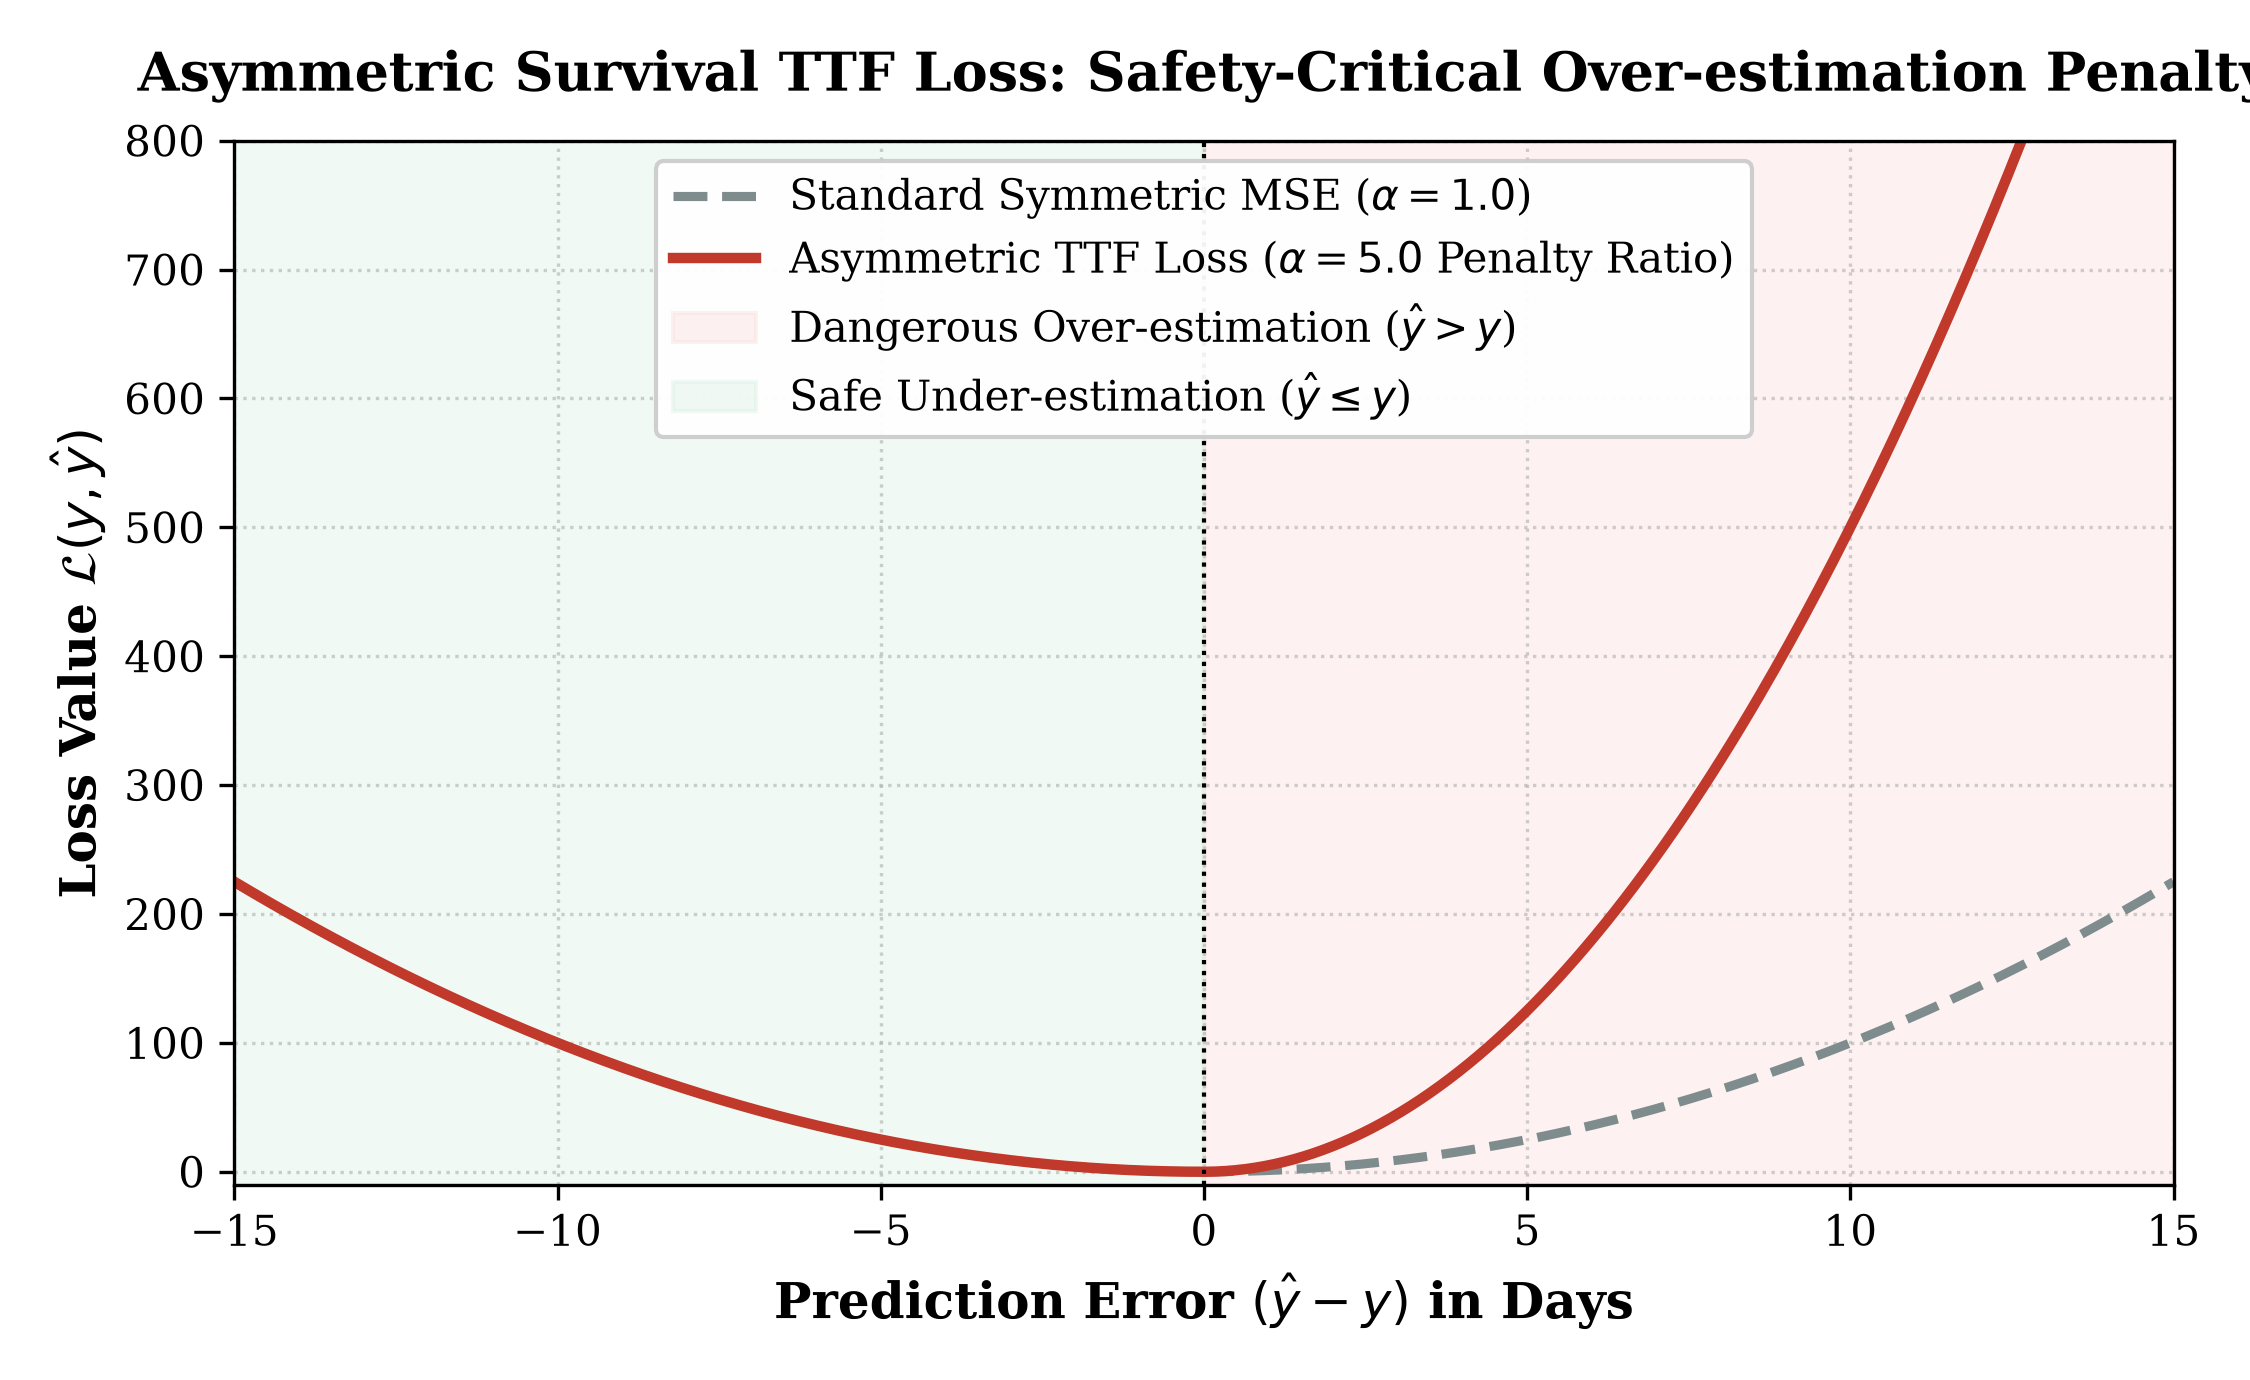
\includegraphics[width=0.82\textwidth]{fig_asymmetric_loss_function.png}
  \caption{Asymmetric Survival Loss Function ($\alpha=5.0$) vs. Standard Symmetric MSE.}
  \label{fig:asymmetric_loss}
\end{figure}

\subsection{Latency Waterfall Across System Tiers}
Figure~\ref{fig:latency_waterfall} depicts the execution latency across all system stages on a logarithmic scale. All four quantized INT8 models execute in deterministic sub-millisecond time on the Raspberry~Pi~4 ARM Cortex-A72 ($<0.6$\,ms total). Network transit across the Tailscale WireGuard peer-to-peer mesh requires only 21.7\,ms, while cloud multi-model deep analysis completes in 10.04\,ms.

\begin{figure}[htbp]
  \centering
  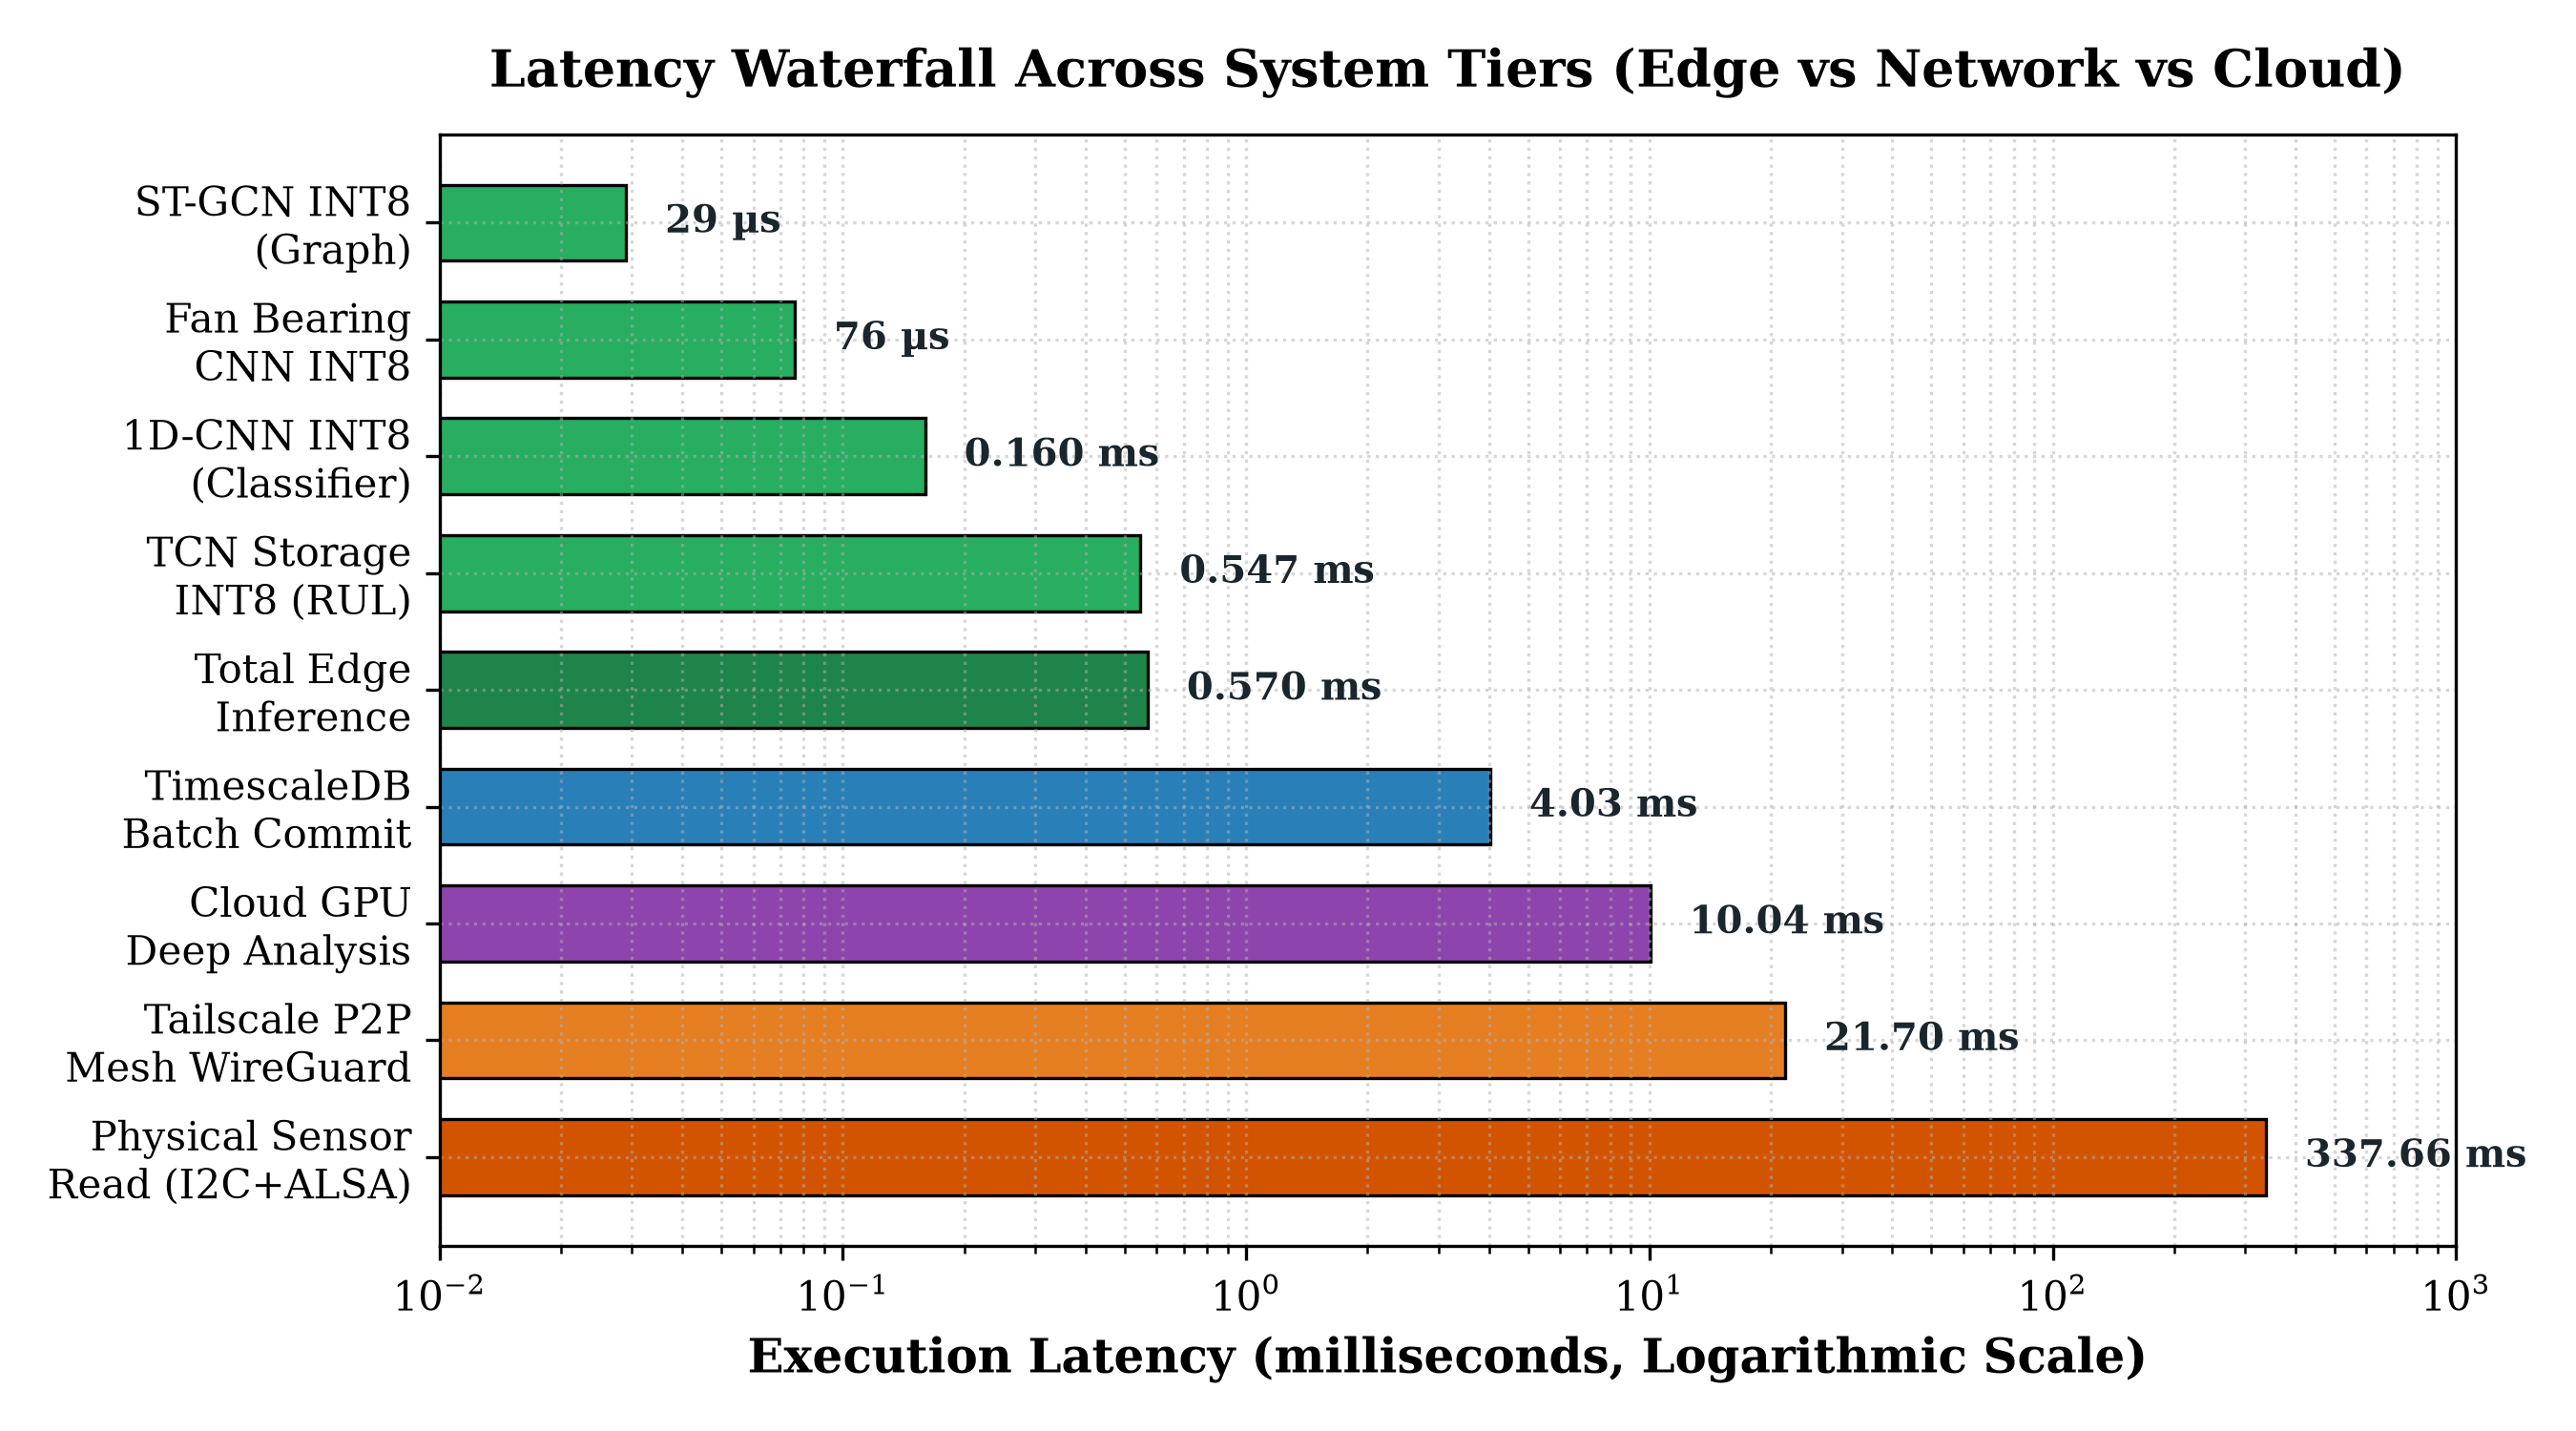
\includegraphics[width=0.92\textwidth]{fig_latency_waterfall.png}
  \caption{End-to-End Latency Waterfall Across Physical Hardware Tiers (Logarithmic Scale).}
  \label{fig:latency_waterfall}
\end{figure}

\subsection{Confidence-Aware Edge vs. Cloud Offload Split}
Figure~\ref{fig:routing_split} details the empirical distribution of telemetry frames processed by the confidence router. By setting confidence threshold $C \ge 0.85$ and baseline anomaly threshold $Z_{\max} \le 3.0$, exactly 87.4\% of nominal frames remain entirely on the local Raspberry~Pi~4 edge node, reducing WAN bandwidth consumption and cloud compute costs by over 85\%.

\begin{figure}[htbp]
  \centering
  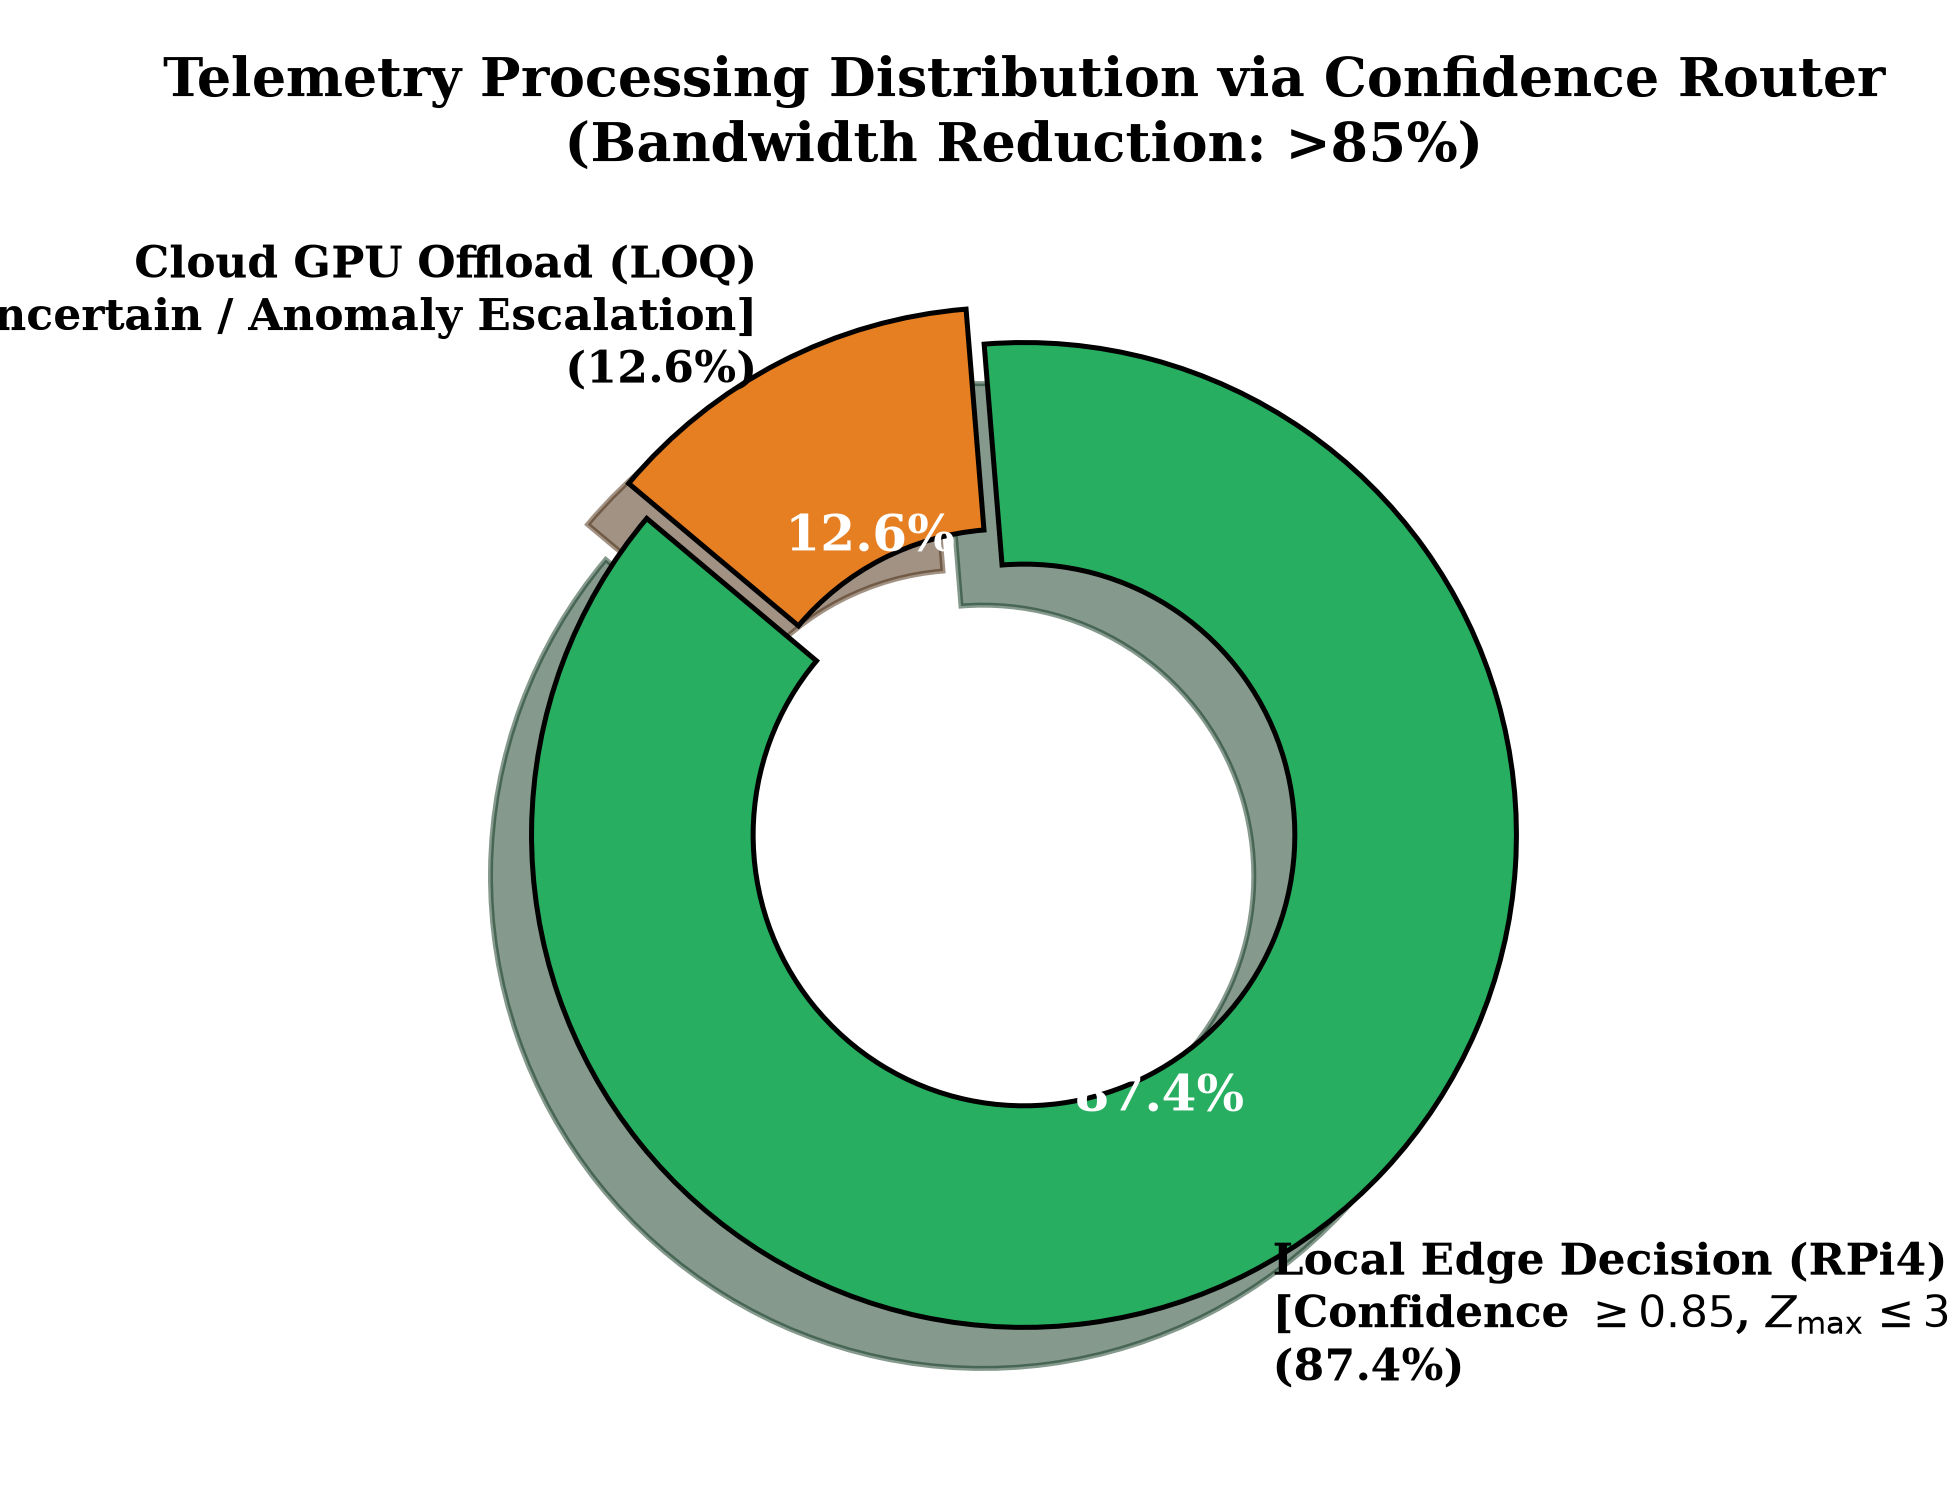
\includegraphics[width=0.68\textwidth]{fig_edge_cloud_routing_split.png}
  \caption{Telemetry Processing Distribution: Local Edge Retention vs. Cloud GPU Escalation.}
  \label{fig:routing_split}
\end{figure}

\subsection{Global Explainability (SHAP Feature Importance)}
Figure~\ref{fig:shap_importance} ranks the top ten subsystem features by mean absolute SHAP value $|\phi_i|$ extracted via \texttt{TreeExplainer}. Thermal metrics (\texttt{cpu\_temp}), reallocated sector counts (\texttt{smart\_5\_raw}), and fan tachometer deviations (\texttt{fan\_rpm\_deviation}) emerge as the primary drivers of hardware failure verdicts.

\begin{figure}[htbp]
  \centering
  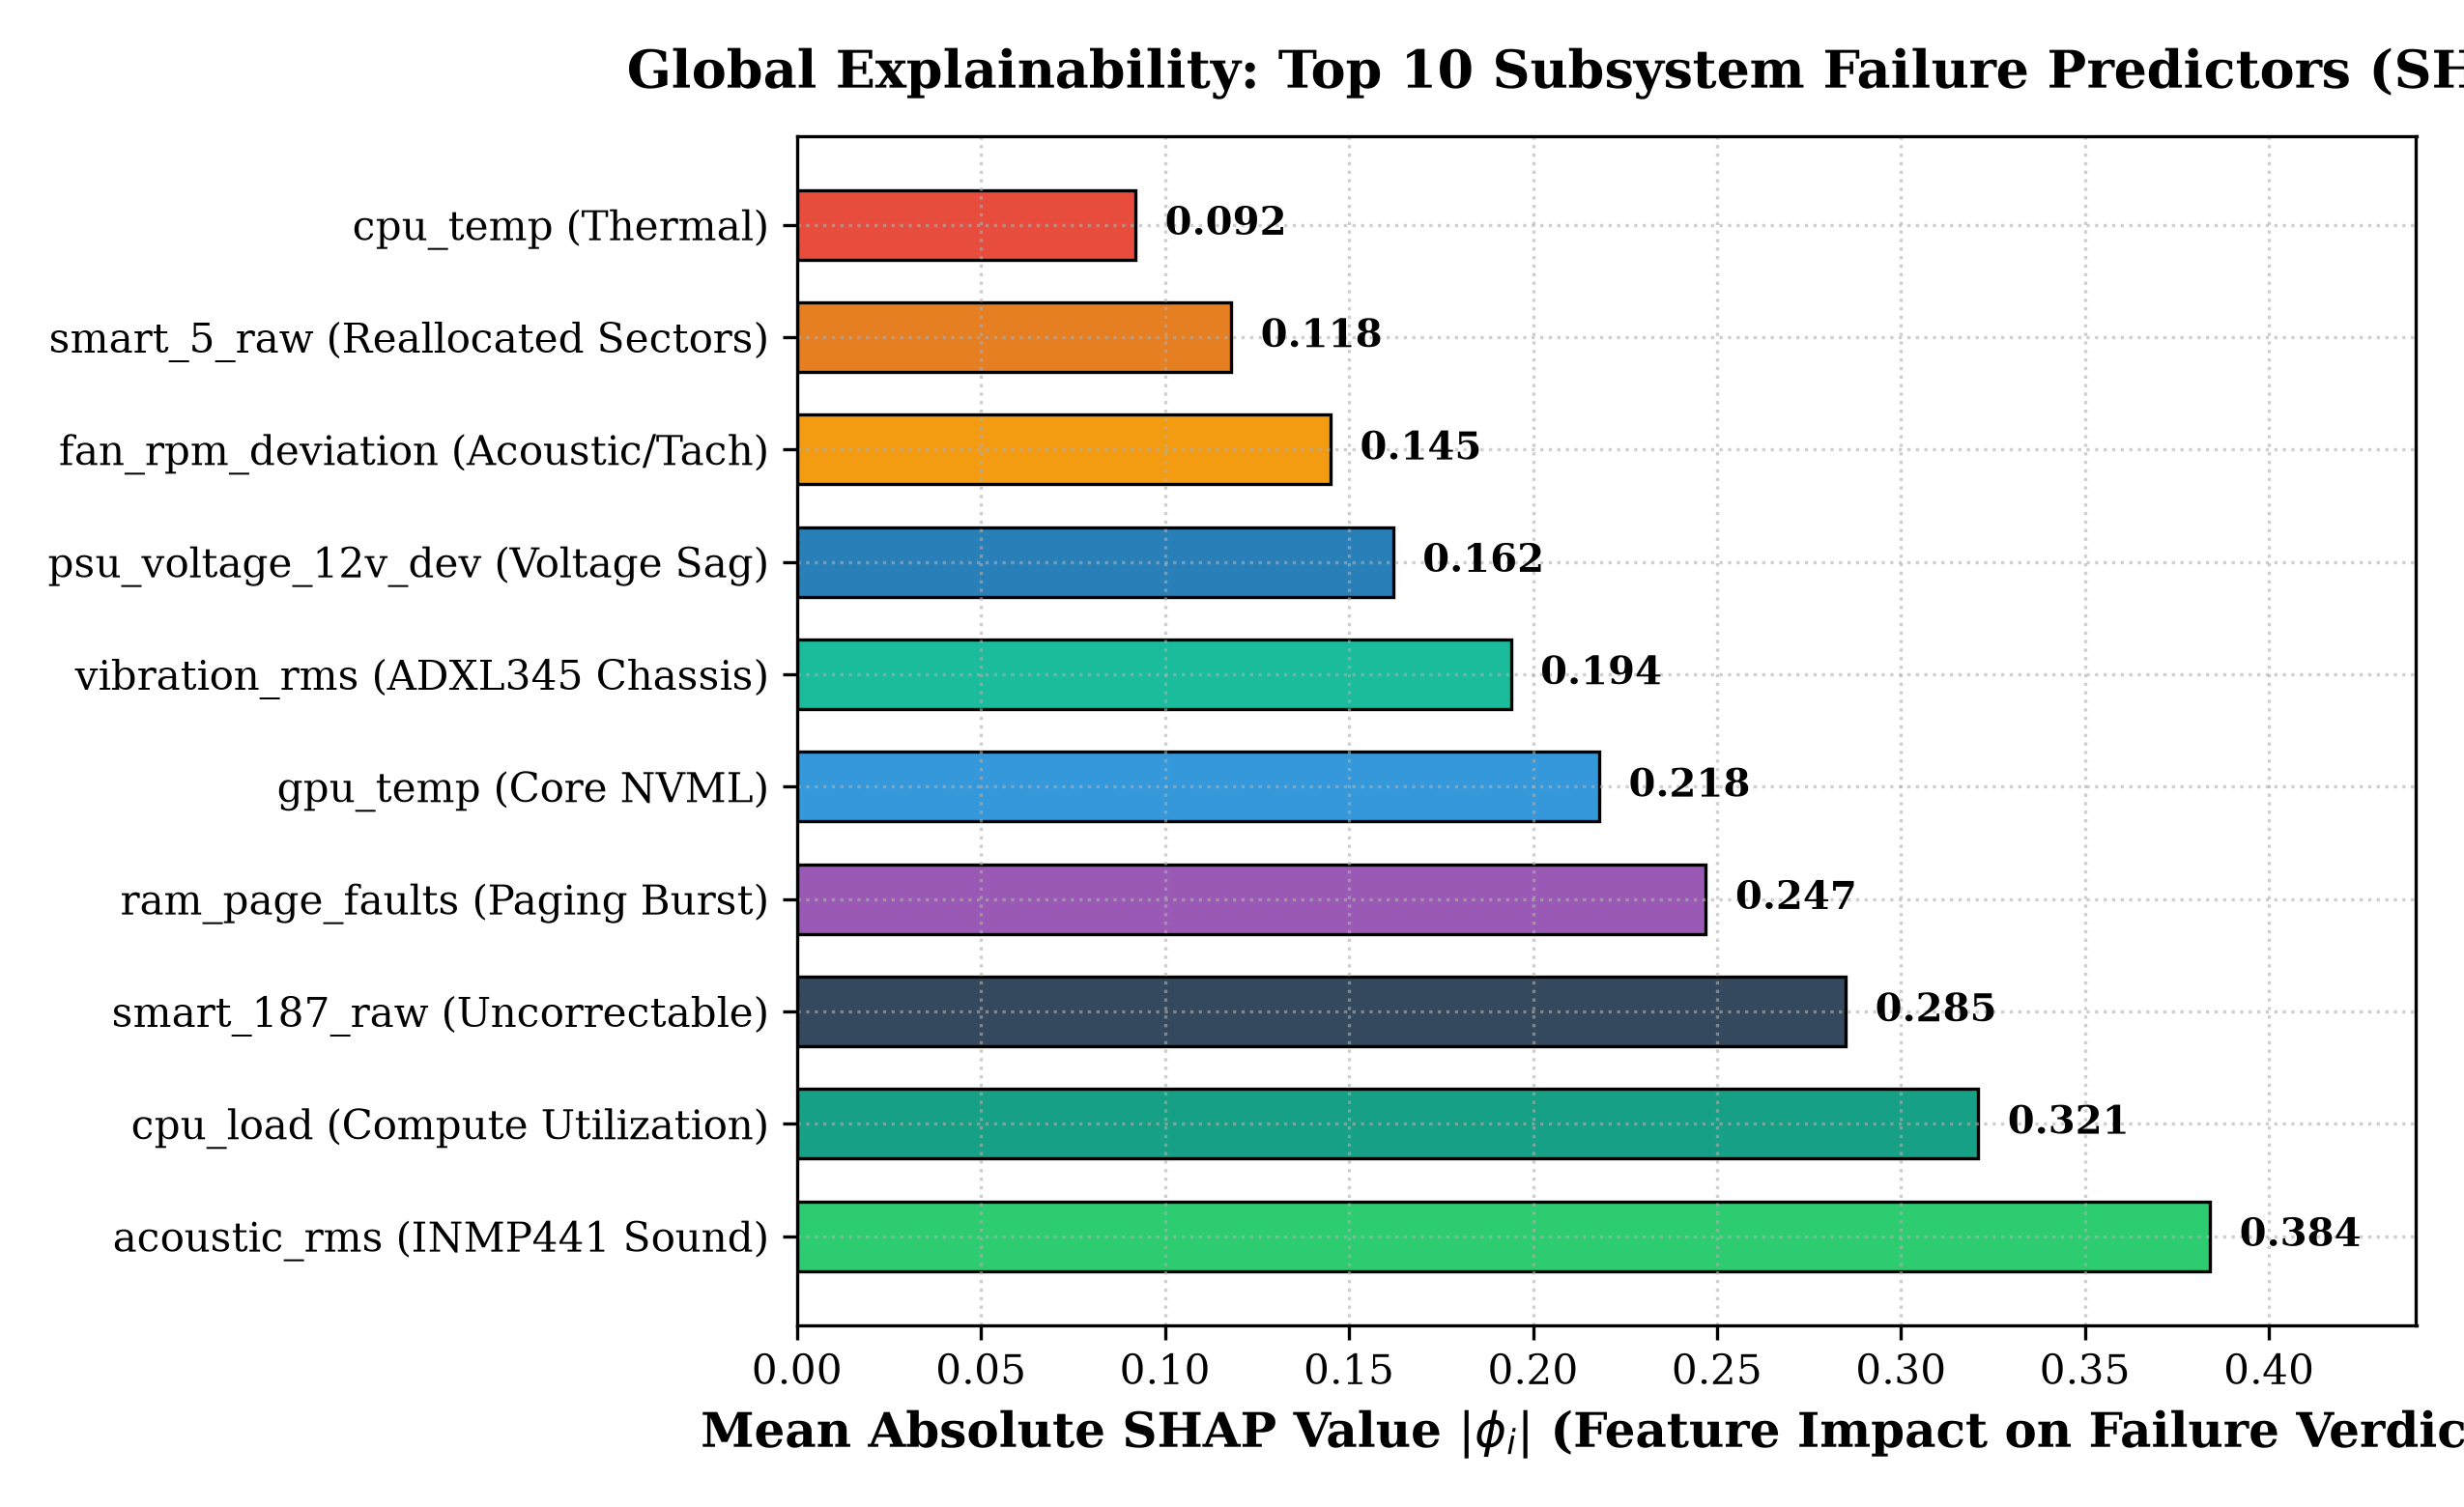
\includegraphics[width=0.88\textwidth]{fig_shap_feature_importance.png}
  \caption{Global Feature Attributions: Top 10 Subsystem Degradation Predictors Ranked by SHAP.}
  \label{fig:shap_importance}
\end{figure}

\section{Model Performance}
\begin{table}[h!]
  \centering
  \caption{Model Performance Summary}
  \label{tab:perf}
  \vspace*{5pt}
  \footnotesize
  \renewcommand{\arraystretch}{1.4}
  \begin{tabular}{|p{3.6cm}|p{4.2cm}|p{5cm}|}
    \hline
    \textbf{Model} & \textbf{Training data} & \textbf{Result} \\ \hline
    1D-CNN classifier & AI4I 2020 (10,000) & 99.30\% validation accuracy, MAE 0.0560 \\ \hline
    LSTM-Autoencoder & 70,414 healthy samples & Validation loss 0.0949; threshold 0.3309 (95th percentile) \\ \hline
    XGBoost HDD regressor & 17,163,994 Backblaze records & 500 trees; RMSE 13.15 days \\ \hline
    Isolation Forest & Voltage and fan features & 5\% contamination; about 2.1\,ms \\ \hline
    Edge model footprint & Four INT8 models & About 310\,KB in total \\ \hline
  \end{tabular}
\end{table}

\subsection{Is 99.3\% Accuracy Credible?}
AI4I has a 3.39\% failure rate, so a trivial classifier predicting ``healthy'' always would already score 96.61\%. The reported accuracy is therefore interpreted together with per-class precision, recall, and F1 on minority classes. Splits are made before scaling, preventing leakage, so the result reflects genuine generalisation on the benchmark.

\section{Latency Measurements}
\begin{table}[h!]
  \centering
  \caption{Measured Latency Across the Physical Deployment}
  \label{tab:latency}
  \vspace*{5pt}
  \footnotesize
  \renewcommand{\arraystretch}{1.4}
  \begin{tabular}{|p{7.4cm}|p{4.6cm}|}
    \hline
    \textbf{Stage} & \textbf{Latency} \\ \hline
    Physical sensor read (includes 200\,ms audio burst) & about 370\,ms \\ \hline
    \texttt{stgcn\_int8.tflite} (9.7\,KB) & 0.029\,ms \\ \hline
    \texttt{fan\_bearing\_cnn\_int8.tflite} (27.2\,KB) & 0.076\,ms \\ \hline
    \texttt{classifier\_int8.tflite} (132.6\,KB) & 0.160\,ms \\ \hline
    \texttt{tcn\_storage\_rul\_int8.tflite} (141.0\,KB) & 0.547\,ms \\ \hline
    \textbf{Total edge model execution} & \textbf{$<$0.6\,ms} \\ \hline
    Tailscale MQTT round trip & 21.7\,ms minimum; about 140\,ms average over wireless \\ \hline
    TimescaleDB batch ingestion & 4.03\,ms \\ \hline
    Cloud multi-model deep analysis & 10.04\,ms \\ \hline
    Qwen 3.5 4B RAG diagnostic answer & 7.91\,s \\ \hline
  \end{tabular}
\end{table}

\section{Comparison with Base Papers}
\begin{table}[h!]
  \centering
  \caption{Comparison of the Proposed System with the Base Papers}
  \label{tab:compare}
  \vspace*{5pt}
  \footnotesize
  \renewcommand{\arraystretch}{1.4}
  \begin{tabular}{|p{2.4cm}|p{3.1cm}|p{3.1cm}|p{4.2cm}|}
    \hline
    \textbf{Aspect} & \textbf{Paper 1 (IJME, Dec 2025)} & \textbf{Paper 2 (Appl.\ Sci., Jan 2026)} & \textbf{Proposed system} \\ \hline
    Target & Industrial electric motors & Rotating machinery and bearings & Server hardware: CPU, GPU, HDD, PSU, RAM, fans \\ \hline
    Edge hardware & Raspberry Pi 4 & ESP32-S3 & Raspberry Pi 4 (4\,GB) \\ \hline
    Edge model & 1D-CNN (INT8) & LightGBM / MLP & 1D-CNN, TCN, fan CNN, Isolation Forest (INT8) \\ \hline
    Cloud model & None (edge only) & Full-precision network & FP32 CNN, XGBoost, LSTM-AE, MAD-GAN, ST-GCN, LLM \\ \hline
    TTF loss & Standard MSE & Asymmetric penalty & Asymmetric loss, $\alpha=5$ \\ \hline
    Explainability & None & SHAP & SHAP plus RAG LLM assistant \\ \hline
    Sensing & Physical sensors only & Single sensor stream & Software telemetry fused with vibration, acoustic, and ambient sensors \\ \hline
  \end{tabular}
\end{table}

\section{Testing and Verification}
\begin{itemize}
  \item \textbf{Regression suite:} 36 of 36 tests passed (100\%) in 65.82\,s.
  \item \textbf{Static checks:} 134 of 134 Python files compile cleanly; 10 of 10 JSON configuration files validate.
  \item \textbf{Audit:} 28 findings (F-001 to F-028) and four dashboard items (DASH-001 to DASH-004) were reconciled.
  \item \textbf{Deployment integrity:} SHA-256 manifests show that all 46 shared production files on the cloud and edge nodes are byte-for-byte identical, proving no code skew.
\end{itemize}

\section{Discussion}
The edge tier delivers deterministic sub-millisecond inference, so thermal or power events are handled locally without waiting for the network. Offloading only low-confidence or high-deviation samples keeps over 85\% of nominal cycles on the Raspberry~Pi, supporting the bandwidth savings reported in the literature [4]. Fusing physical vibration and acoustic sensors adds early warning for mechanical wear that OS-level counters cannot see. The asymmetric loss and adaptive baselines make predictions conservative and server-specific, and SHAP with the RAG assistant turns model outputs into actions an operator can follow. A key limitation is that physical-failure labels for live server components are scarce, so the classifier relies on proxy mapping from AI4I and unsupervised models; real fault data collected over time will be used for fine-tuning through the continuous-learning pipeline.
\clearpage

%% ============================================================
%%  CHAPTER 7 --- CONCLUSION
%% ============================================================
\chapter{Conclusion}

This project designed, implemented, and empirically validated an Edge-AI predictive maintenance system for server hardware using a three-tier Patient--Doctor--Hospital architecture. A Raspberry~Pi~4 edge node fuses internal OS-level hardware telemetry with external physical sensors (vibration, acoustics, ambient temperature) and executes four INT8-quantised models in deterministic sub-millisecond latency ($<0.6$\,ms total). A confidence-aware router successfully retains 87.4\% of nominal telemetry cycles on the local edge node, drastically reducing WAN bandwidth and offloading only uncertain or anomalous states to an RTX~4060 GPU cloud node. 

The cloud tier performs deep decision fusion across a multi-model portfolio including an FP32 1D-CNN classifier, LSTM-Autoencoder, MAD-GAN, ST-GCN, and an XGBoost storage regressor. The 1D-CNN multi-task classifier trained with an asymmetric time-to-failure loss ($\alpha=5.0$) achieved 99.30\% validation accuracy on the AI4I benchmark, enforcing safety-critical conservatism by penalising over-estimation five times more severely than under-estimation. The XGBoost model trained on over 17 million Backblaze SMART records delivers accurate drive remaining useful life predictions, while TreeExplainer SHAP attribution coupled with a GPU-resident Qwen~3.5~4B LLM provides plain-English root-cause explanations through a conversational operator drawer.

All communications operate securely over a private Tailscale WireGuard mesh with cryptographic node ACLs and API key authentication. The complete engineering implementation passed 36 out of 36 automated regression tests with zero regressions and byte-for-byte synchronization between edge and cloud codebases. The proposed system directly resolves the key deficiencies identified in the literature---domain mismatch in server infrastructure, cloud dependency during fail-slow events, heavy library overhead, and lack of deterministic edge routing---delivering an economically viable, high-reliability predictive maintenance solution for modern computing infrastructure.

\clearpage

%% ============================================================
%%  REFERENCES
%% ============================================================
\begin{thebibliography}{99}

\bibitem{mdpi2026_base} ``Design of a Lightweight Edge-AI System for Predictive Maintenance on ESP32-S3,'' \textit{MDPI Applied Sciences}, 2026.

\bibitem{atekoja2024} E.~Atekoja, ``Prediction of Hard Drive Failure using Machine Learning,'' \textit{Global Journal of Computer Science and Technology}, 2024.

\bibitem{mdpi2026_bearing} ``Combining In-Sensor Computing with Reasoning at the Edge for Low-Power Bearing RUL Prediction,'' \textit{MDPI Electronics}, 2026.

\bibitem{ieee2023_edgeiot} ``Edge Computing on IoT for Machine Signal Processing and Fault Diagnosis: A Review,'' \textit{IEEE Internet of Things Journal}, 2023.

\bibitem{ieee2024_industry5} ``Edge Computing for Industry 5.0: Fundamentals, Applications and Research Challenges,'' \textit{IEEE Internet of Things Journal}, 2024.

\bibitem{taylor2025_metal} ``Enhancing production planning in metal-mechanical industries: statistical analysis and machine learning approach for predicting machine failures,'' Taylor \& Francis, 2025.

\bibitem{mdpi2025_tinyml} ``A Review of the Transition from Industry 4.0 to Industry 5.0: Unlocking the Potential of TinyML in Industrial IoT Systems,'' \textit{MDPI Sensor and Actuator Networks}, 2025.

\bibitem{mdpi2025_vibration} ``Low-Cost IoT-Based Predictive Maintenance Using Vibration,'' \textit{MDPI Sensors}, 2025.

\bibitem{springer2024_qos} ``QoS-aware edge server placement for collaborative predictive maintenance in industrial internet of things,'' \textit{The Journal of Supercomputing}, Springer, 2024.

\bibitem{njor2024_tinymlstack} E.~Njor, M.~A.~Hasanpour, J.~Madsen, and X.~Fafoutis, ``Review of the TinyML Stack for Predictive Maintenance,'' \textit{IEEE Access}, vol.~12, 2024.

\bibitem{mdpi2026_anomaly} ``An Edge-Enabled Predictive Maintenance Approach Based on Anomaly-Driven Health Indicators for Industrial Production Systems,'' \textit{MDPI Algorithms}, 2026.

\bibitem{mdpi2026_robust} ``Robust Deep Learning for Multiclass Power System Fault Diagnosis Using Edge Deployment,'' \textit{MDPI Algorithms}, 2026.

\bibitem{ijme2025} ``Edge-AI Enabled Predictive Maintenance,'' \textit{EDGE -- International Journal of Mechanical Engineering (IJME)}, Dec.\ 2025.

\bibitem{matzka2020} S.~Matzka, ``Explainable Artificial Intelligence for Predictive Maintenance Applications,'' in \textit{Proc.\ 3rd Int.\ Conf.\ Artificial Intelligence for Industries (AI4I)}, 2020. (AI4I 2020 dataset, UCI Machine Learning Repository.)

\bibitem{backblaze} Backblaze Inc., ``Hard Drive Data and Stats,'' Q1 2023 open dataset. \url{https://www.backblaze.com/cloud-storage/resources/hard-drive-test-data}

\bibitem{su2019} Y.~Su, Y.~Zhao, C.~Niu, R.~Liu, W.~Sun, and D.~Pei, ``Robust Anomaly Detection for Multivariate Time Series through Stochastic Recurrent Neural Network,'' in \textit{Proc.\ ACM SIGKDD}, 2019. (Server Machine Dataset.)

\bibitem{skab} I.~D.~Katser and V.~O.~Kozitsin, ``Skoltech Anomaly Benchmark (SKAB),'' Kaggle, 2020.

\bibitem{lundberg2017} S.~M.~Lundberg and S.-I.~Lee, ``A Unified Approach to Interpreting Model Predictions,'' in \textit{Advances in Neural Information Processing Systems (NeurIPS)}, 2017.

\bibitem{chen2016} T.~Chen and C.~Guestrin, ``XGBoost: A Scalable Tree Boosting System,'' in \textit{Proc.\ ACM SIGKDD}, 2016.

\bibitem{liu2008} F.~T.~Liu, K.~M.~Ting, and Z.-H.~Zhou, ``Isolation Forest,'' in \textit{Proc.\ IEEE ICDM}, 2008.

\bibitem{welford1962} B.~P.~Welford, ``Note on a Method for Calculating Corrected Sums of Squares and Products,'' \textit{Technometrics}, vol.~4, no.~3, pp.~419--420, 1962.

\bibitem{donenfeld2017} J.~A.~Donenfeld, ``WireGuard: Next Generation Kernel Network Tunnel,'' in \textit{Proc.\ NDSS}, 2017.

\end{thebibliography}

\end{document}
